% Options for packages loaded elsewhere
\PassOptionsToPackage{unicode}{hyperref}
\PassOptionsToPackage{hyphens}{url}
%
\documentclass[
  ignorenonframetext,
]{beamer}
\usepackage{pgfpages}
\setbeamertemplate{caption}[numbered]
\setbeamertemplate{caption label separator}{: }
\setbeamercolor{caption name}{fg=normal text.fg}
\beamertemplatenavigationsymbolsempty
% Prevent slide breaks in the middle of a paragraph
\widowpenalties 1 10000
\raggedbottom
\setbeamertemplate{part page}{
  \centering
  \begin{beamercolorbox}[sep=16pt,center]{part title}
    \usebeamerfont{part title}\insertpart\par
  \end{beamercolorbox}
}
\setbeamertemplate{section page}{
  \centering
  \begin{beamercolorbox}[sep=12pt,center]{part title}
    \usebeamerfont{section title}\insertsection\par
  \end{beamercolorbox}
}
\setbeamertemplate{subsection page}{
  \centering
  \begin{beamercolorbox}[sep=8pt,center]{part title}
    \usebeamerfont{subsection title}\insertsubsection\par
  \end{beamercolorbox}
}
\AtBeginPart{
  \frame{\partpage}
}
\AtBeginSection{
  \ifbibliography
  \else
    \frame{\sectionpage}
  \fi
}
\AtBeginSubsection{
  \frame{\subsectionpage}
}
\usepackage{lmodern}
\usepackage{amssymb,amsmath}
\usepackage{ifxetex,ifluatex}
\ifnum 0\ifxetex 1\fi\ifluatex 1\fi=0 % if pdftex
  \usepackage[T1]{fontenc}
  \usepackage[utf8]{inputenc}
  \usepackage{textcomp} % provide euro and other symbols
\else % if luatex or xetex
  \usepackage{unicode-math}
  \defaultfontfeatures{Scale=MatchLowercase}
  \defaultfontfeatures[\rmfamily]{Ligatures=TeX,Scale=1}
\fi
% Use upquote if available, for straight quotes in verbatim environments
\IfFileExists{upquote.sty}{\usepackage{upquote}}{}
\IfFileExists{microtype.sty}{% use microtype if available
  \usepackage[]{microtype}
  \UseMicrotypeSet[protrusion]{basicmath} % disable protrusion for tt fonts
}{}
\makeatletter
\@ifundefined{KOMAClassName}{% if non-KOMA class
  \IfFileExists{parskip.sty}{%
    \usepackage{parskip}
  }{% else
    \setlength{\parindent}{0pt}
    \setlength{\parskip}{6pt plus 2pt minus 1pt}}
}{% if KOMA class
  \KOMAoptions{parskip=half}}
\makeatother
\usepackage{xcolor}
\IfFileExists{xurl.sty}{\usepackage{xurl}}{} % add URL line breaks if available
\IfFileExists{bookmark.sty}{\usepackage{bookmark}}{\usepackage{hyperref}}
\hypersetup{
  pdftitle={MA8701 Advanced methods in statistical inference and learning},
  pdfauthor={Mette Langaas IMF/NTNU},
  hidelinks,
  pdfcreator={LaTeX via pandoc}}
\urlstyle{same} % disable monospaced font for URLs
\newif\ifbibliography
\usepackage{color}
\usepackage{fancyvrb}
\newcommand{\VerbBar}{|}
\newcommand{\VERB}{\Verb[commandchars=\\\{\}]}
\DefineVerbatimEnvironment{Highlighting}{Verbatim}{commandchars=\\\{\}}
% Add ',fontsize=\small' for more characters per line
\usepackage{framed}
\definecolor{shadecolor}{RGB}{248,248,248}
\newenvironment{Shaded}{\begin{snugshade}}{\end{snugshade}}
\newcommand{\AlertTok}[1]{\textcolor[rgb]{0.94,0.16,0.16}{#1}}
\newcommand{\AnnotationTok}[1]{\textcolor[rgb]{0.56,0.35,0.01}{\textbf{\textit{#1}}}}
\newcommand{\AttributeTok}[1]{\textcolor[rgb]{0.77,0.63,0.00}{#1}}
\newcommand{\BaseNTok}[1]{\textcolor[rgb]{0.00,0.00,0.81}{#1}}
\newcommand{\BuiltInTok}[1]{#1}
\newcommand{\CharTok}[1]{\textcolor[rgb]{0.31,0.60,0.02}{#1}}
\newcommand{\CommentTok}[1]{\textcolor[rgb]{0.56,0.35,0.01}{\textit{#1}}}
\newcommand{\CommentVarTok}[1]{\textcolor[rgb]{0.56,0.35,0.01}{\textbf{\textit{#1}}}}
\newcommand{\ConstantTok}[1]{\textcolor[rgb]{0.00,0.00,0.00}{#1}}
\newcommand{\ControlFlowTok}[1]{\textcolor[rgb]{0.13,0.29,0.53}{\textbf{#1}}}
\newcommand{\DataTypeTok}[1]{\textcolor[rgb]{0.13,0.29,0.53}{#1}}
\newcommand{\DecValTok}[1]{\textcolor[rgb]{0.00,0.00,0.81}{#1}}
\newcommand{\DocumentationTok}[1]{\textcolor[rgb]{0.56,0.35,0.01}{\textbf{\textit{#1}}}}
\newcommand{\ErrorTok}[1]{\textcolor[rgb]{0.64,0.00,0.00}{\textbf{#1}}}
\newcommand{\ExtensionTok}[1]{#1}
\newcommand{\FloatTok}[1]{\textcolor[rgb]{0.00,0.00,0.81}{#1}}
\newcommand{\FunctionTok}[1]{\textcolor[rgb]{0.00,0.00,0.00}{#1}}
\newcommand{\ImportTok}[1]{#1}
\newcommand{\InformationTok}[1]{\textcolor[rgb]{0.56,0.35,0.01}{\textbf{\textit{#1}}}}
\newcommand{\KeywordTok}[1]{\textcolor[rgb]{0.13,0.29,0.53}{\textbf{#1}}}
\newcommand{\NormalTok}[1]{#1}
\newcommand{\OperatorTok}[1]{\textcolor[rgb]{0.81,0.36,0.00}{\textbf{#1}}}
\newcommand{\OtherTok}[1]{\textcolor[rgb]{0.56,0.35,0.01}{#1}}
\newcommand{\PreprocessorTok}[1]{\textcolor[rgb]{0.56,0.35,0.01}{\textit{#1}}}
\newcommand{\RegionMarkerTok}[1]{#1}
\newcommand{\SpecialCharTok}[1]{\textcolor[rgb]{0.00,0.00,0.00}{#1}}
\newcommand{\SpecialStringTok}[1]{\textcolor[rgb]{0.31,0.60,0.02}{#1}}
\newcommand{\StringTok}[1]{\textcolor[rgb]{0.31,0.60,0.02}{#1}}
\newcommand{\VariableTok}[1]{\textcolor[rgb]{0.00,0.00,0.00}{#1}}
\newcommand{\VerbatimStringTok}[1]{\textcolor[rgb]{0.31,0.60,0.02}{#1}}
\newcommand{\WarningTok}[1]{\textcolor[rgb]{0.56,0.35,0.01}{\textbf{\textit{#1}}}}
\usepackage{graphicx,grffile}
\makeatletter
\def\maxwidth{\ifdim\Gin@nat@width>\linewidth\linewidth\else\Gin@nat@width\fi}
\def\maxheight{\ifdim\Gin@nat@height>\textheight\textheight\else\Gin@nat@height\fi}
\makeatother
% Scale images if necessary, so that they will not overflow the page
% margins by default, and it is still possible to overwrite the defaults
% using explicit options in \includegraphics[width, height, ...]{}
\setkeys{Gin}{width=\maxwidth,height=\maxheight,keepaspectratio}
% Set default figure placement to htbp
\makeatletter
\def\fps@figure{htbp}
\makeatother
\setlength{\emergencystretch}{3em} % prevent overfull lines
\providecommand{\tightlist}{%
  \setlength{\itemsep}{0pt}\setlength{\parskip}{0pt}}
\setcounter{secnumdepth}{-\maxdimen} % remove section numbering

\title{MA8701 Advanced methods in statistical inference and learning}
\subtitle{L2: Shrinkage - the beginning}
\author{Mette Langaas IMF/NTNU}
\date{17 January, 2021}

\begin{document}
\frame{\titlepage}

\begin{frame}

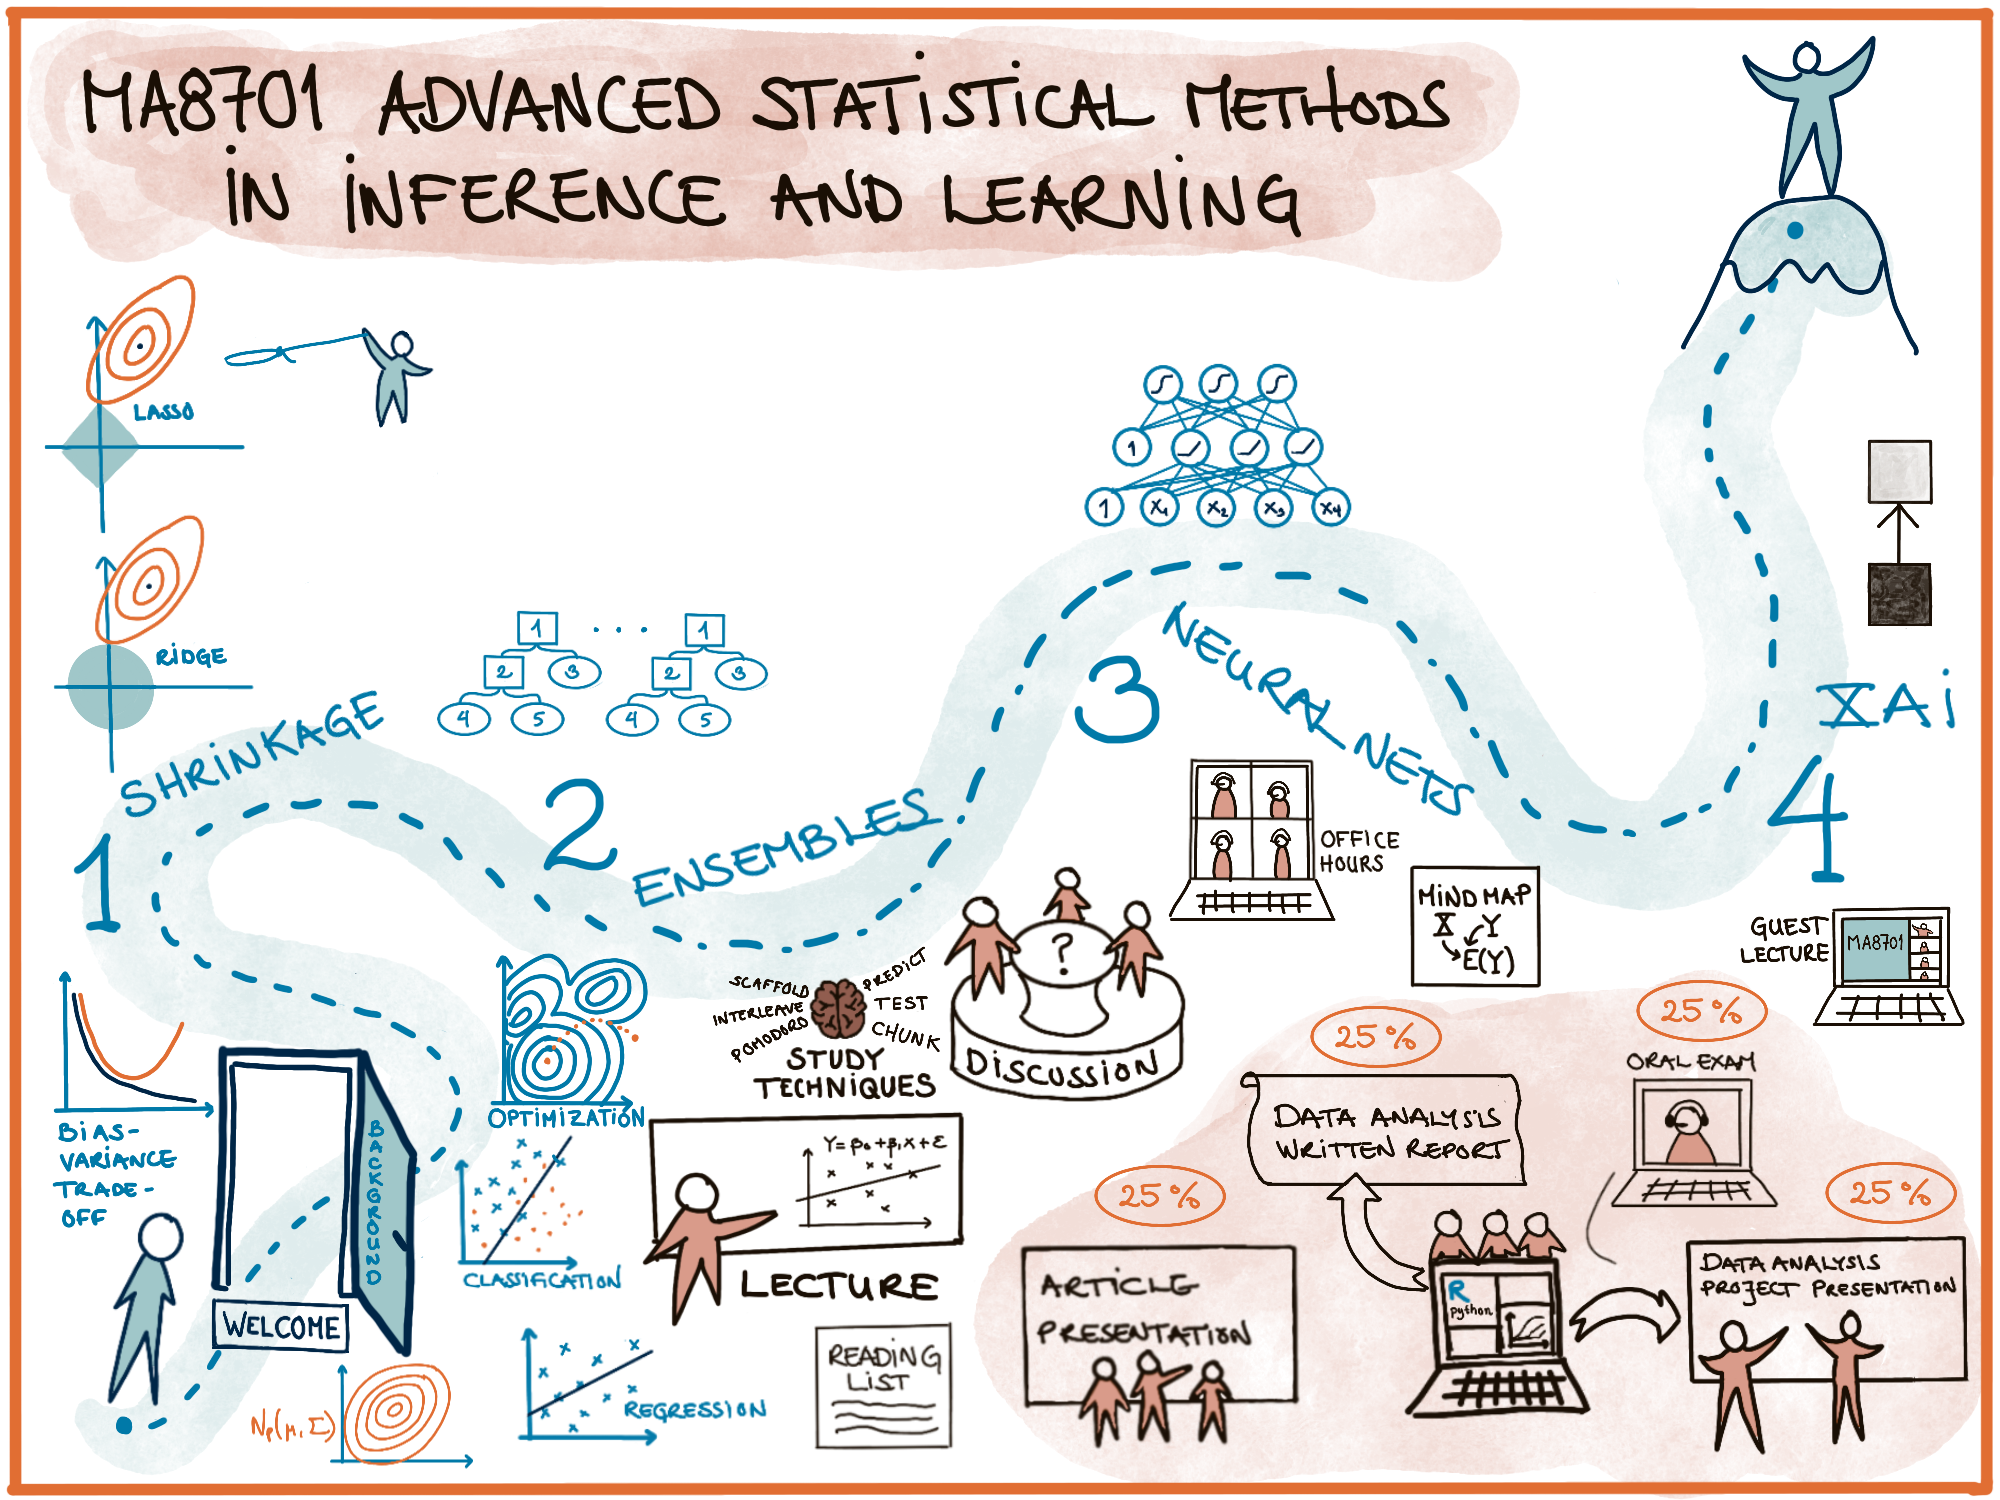
\includegraphics{../overviewv2.png}

\end{frame}

\begin{frame}{Shrinkage}
\protect\hypertarget{shrinkage}{}

\begin{block}{Literature lecture 2 (L2)}

\begin{itemize}
\item
  {[}ELS{]} The Elements of Statistical Learning: Data Mining,
  Inference, and Prediction, Second Edition (Springer Series in
  Statistics, 2009) by Trevor Hastie, Robert Tibshirani, and Jerome
  Friedman.
  \href{https://web.stanford.edu/~hastie/Papers/ESLII.pdf}{Ebook}.
  Chapter 3.2 and 3.4.1-3.4.3.
\item
  {[}HTW{]} Hastie, Tibshirani, Wainwrigh: ``Statistical Learning with
  Sparsity: The Lasso and Generalizations''. CRC press.
  \href{https://trevorhastie.github.io/}{Ebook}. Chapter 1, 2.1-2.3,2.5.
\end{itemize}

and for the interested student

\begin{itemize}
\tightlist
\item
  \href{https://arxiv.org/pdf/1509.09169.pdf}{Wessel N. van Wieringen:
  Lecture notes on ridge regression} (We will refer to this note as WNvW
  below.)
\end{itemize}

Some figures are taken from An Introduction to Statistical Learning,
with applications in R (Springer, 2013) with permission from the
authors: G. James, D. Witten, T. Hastie and R. Tibshirani.

\end{block}

\end{frame}

\begin{frame}

\begin{block}{What is in a name?}

This part of the course could have been called:

\begin{itemize}
\tightlist
\item
  ``Regularized linear and generalized linear models''
\item
  ``Penalized maximum likelihood estimation''
\item
  and also ``Sparse models'',
\end{itemize}

but it is called ``Shrinkage''.

Focus is on generalized linear models, but we will also consider
shrinkage in the next parts of this course (then for ``more complex''
method).

\textbf{Question:} in linear models (linear regression, generalized
linear regression) we mainly work with methods where parameter estimates
are unbiased - but might have high variance and not give very good
prediction performance overall. Can we use penalization (shrinkage) to
produce parameter estimates with some bias but less variance, so that
the prediction performance is improved?

\end{block}

\end{frame}

\begin{frame}

We will look at different ways of penalization (which produces shrunken
estimators) - mainly what is called ridge and lasso methods.

Ridge is not a sparse method, but lasso is. In sparse statistical models
a \emph{small number of covariates} play an important role.

HTW (page 2): \emph{Bet on sparsity principle: Use a procedure that does
well in sparse problems, since no procedure does well in dense
problems.}

Shrinkage (penalization, regularization) methods are especially suitable
in situations where we have multi-collinearity and/or more covariates
than observations \(N<<p\). Two examples are

\begin{itemize}
\tightlist
\item
  in medicine with genetic data, where the number of patient samples is
  less than the number of genetic markers studied,
\item
  in analysis of text (more to come in L3)
\end{itemize}

\end{frame}

\begin{frame}{Linear models}
\protect\hypertarget{linear-models}{}

(ELS 3.2, HTW Ch 2.1)

We will only consider linear models in L2, and move to generalized
linear models in L3.

\begin{block}{Set-up}

Random response \(Y\) and \(p\)-dimensional (random) covariates \(X\).

Training data: \(N\) (independent) observations: \((y_i,x_i)\), where
\(x_i\) is a column vector with \(p\) covariates (features).

\end{block}

\end{frame}

\begin{frame}

\begin{block}{Linear regression model}

(ELS 3.2)

Additive noise model \[ Y=f(X)+\varepsilon\] with
\(\text{E}(\varepsilon)=0\) and \(\text{Var}(\varepsilon)=\sigma^2\).

With squared loss, we remember that the optimal
\(f(X)=\text{E}(Y \mid X)\).

Linear regression model - we assumes that
\[f(X)=\beta_0+\sum_{j=1}^p X_{j}\beta_j \] is linear in \(X\), or that
is a good approximation.

The unknown parameters are the regression coefficients
\(\beta_0,\ldots,\beta_p\) and the error variance
\(\sigma^2_{\varepsilon}\).

From TMA4267 we know that if \((X,Y)\) is jointly multivariate normal,
then the conditional distribution of \(Y\mid X\) has mean that is linear
in \(X\) and variance that is independent of \(X\). Brush-up: See
classnotes
\href{https://www.math.ntnu.no/emner/TMA4267/2017v/TMA4267V2017Part2.pdf}{page
8}.

\end{block}

\end{frame}

\begin{frame}

\begin{figure}
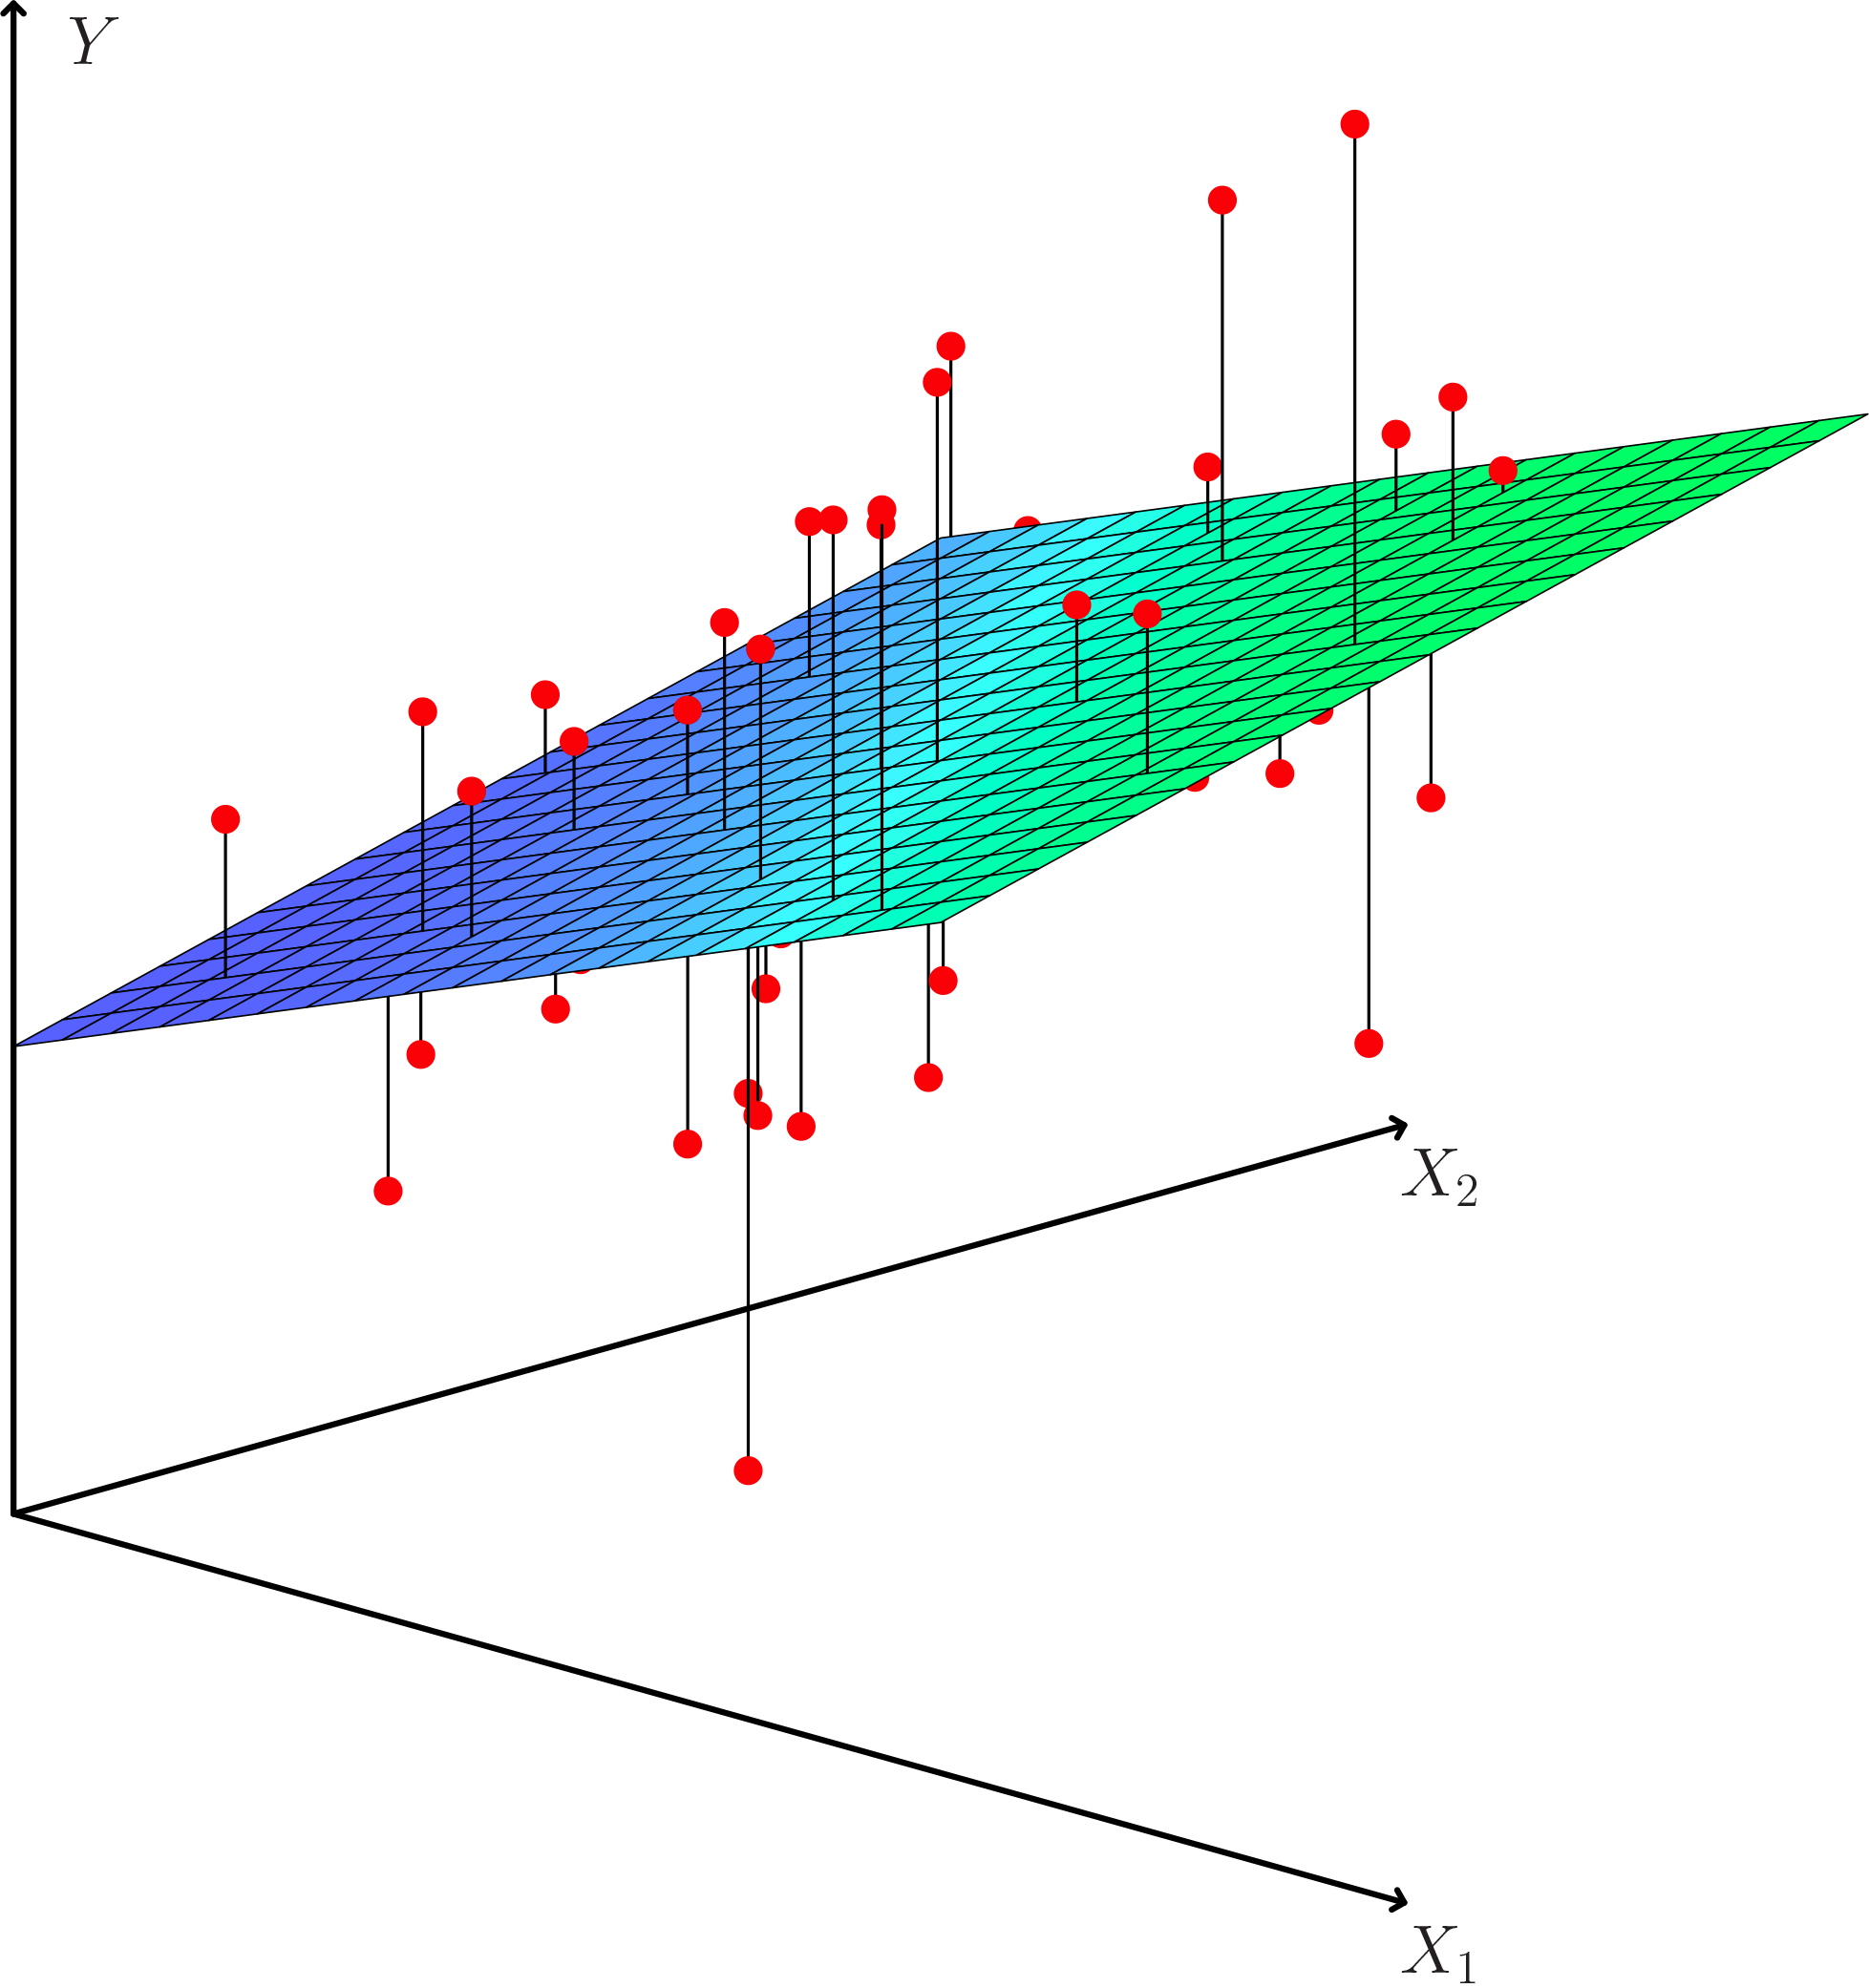
\includegraphics[width=0.5\linewidth]{./ILS34} \caption{Figure from An Introduction to Statistical Learning, with applications in R (Springer, 2013) with permission from the authors: G. James, D. Witten, T. Hastie and R. Tibshirani.}\label{fig:unnamed-chunk-2}
\end{figure}

\end{frame}

\begin{frame}

\begin{block}{Covariates}

The covariates \(X\) can be both quantitative or qualitative, be made of
basis expansions or interactions - and more. For qualitative covariates
often a dummy variable coding is used. Brush-up: See
\href{https://www.math.ntnu.no/emner/TMA4315/2018h/2MLR.html\#categorical_covariates_-_dummy_and_effect_coding}{TMA4315
GLM Module 2}.

For now we don´t say so much more, but later we want the covariates to
be standardized and the reponse to be centered.

\end{block}

\end{frame}

\begin{frame}

\begin{block}{The classical linear model and least squares estimation}

\begin{block}{First version}

For the classical linear model we assume

\[ Y_i=\beta_0+\sum_{j=1}^p X_{j}\beta_j+\varepsilon_i\] with
\(\text{E}(\varepsilon_i)=0\) and
\(\text{Var}(\varepsilon_)=\sigma^2_{\varepsilon}\), and independence of
errors \(\varepsilon_j,\varepsilon_i\).

Regression parameters
\(\beta=(\beta_0,\beta_1,\ldots,\beta_p)\in \Re^{(p+1)}\).

We will use the word \emph{linear predictor}
\(\eta(x_i)=\beta_0+\sum_{j=1}^p x_{ij}\beta_j\), for the linear
combination in the parameters \(\beta\).

The least squares estimator for the parameters \(\beta\) is found by
minimizing the squared-error loss:

\[ \text{minimize}_{\beta} \{ \sum_{i=1}^N (y_i-\beta_0+\sum_{j=1}^p x_{ij}\beta_j)^2\}\]

\end{block}

\end{block}

\end{frame}

\begin{frame}

\begin{block}{Second version}

This can also be written with vectors and matrices for the
\(i=1,\ldots,N\) observations.

\[{\bf Y=X \boldsymbol{\beta}}+{\bf\varepsilon}\] where \({\bf Y}\) is a
\(N \times 1\) random column vector, \({\bf X}\) a \(N \times (p+1)\)
design matrix with row for observations and columns for covariates, and
\({\bf{\varepsilon}}\) \(N \times 1\) random column vector

The assumptions for the classical linear model is:

\begin{enumerate}
\item
  \(\text{E}(\bf{\varepsilon})=\bf{0}\).
\item
  \(\text{Cov}(\varepsilon)=\text{E}(\varepsilon \varepsilon^T)=\sigma^2\bf{I}\).
\item
  The design matrix has full rank, \(\text{rank}({\bf X})=(p+1)\).
\end{enumerate}

\end{block}

\end{frame}

\begin{frame}

The classical \emph{normal} linear regression model is obtained if
additionally

\begin{enumerate}
\setcounter{enumi}{3}
\tightlist
\item
  \(\varepsilon\sim N_n(\bf{0},\sigma^2\bf{I})\) holds.
\end{enumerate}

For random covariates these assumptions are to be understood
conditionally on \(\bf{X}\).

For derivation of the least squares estimator \(\hat{\beta}\) see
\href{https://www.math.ntnu.no/emner/TMA4268/2019v/3LinReg/3LinReg.html\#parameter_estimation}{TMA4268
Module 3} and links therein.

The same results are found using likelihood theory, if we assume that
\(Y\sim N\). See
\href{https://www.math.ntnu.no/emner/TMA4315/2018h/2MLR.html\#likelihood_theory_(from_b4)}{TMA4315
GLM Module 2}. Both methods are written out in
\href{https://www.math.ntnu.no/emner/TMA4268/2018v/notes/LeastSquaresMLR.pdf}{these
class notes from TMA4267/8}.

\end{frame}

\begin{frame}

The squared error loss to be minimized can be written
\[({\bf Y}-{\bf X}{{\beta}})^T({\bf Y}-{\bf X}{{\beta}})\]
Differensiation with respect to the unknown parameter vector, and
equating to zero leads to the \emph{normal equations}.

\[ {\bf X}^T{\bf X}{\beta}= {\bf X}^T {\bf Y}\] To give
\[ \hat{\beta}_{\text LS}=({\bf X}^T{\bf X})^{-1} {\bf X}^T {\bf Y}\]

\end{frame}

\begin{frame}

\begin{block}{Properties of estimators}

If we only assume a classical linear model, the mean and covariance of
\(\hat{\beta}\) is \(\text{E}(\hat{\beta}_{\text LS})=\beta\) and
\(\text{Cov}(\hat{\beta}_{\text LS})=\sigma^2({\bf X}^T{\bf X})^{-1}\).

For the classical normal linear model:

\begin{itemize}
\item
  Least squares and maximum likelihood estimator for \({\bf \beta}\):
  \[ \hat{\beta}_{\text LS}=({\bf X}^T{\bf X})^{-1} {\bf X}^T {\bf Y}\]
  with
  \(\hat{\beta}_{\text LS}\sim N_{p}(\beta,\sigma^2({\bf X}^T{\bf X})^{-1})\).
\item
  Restricted maximum likelihood estimator for \({\bf \sigma}^2\):
  \[ \hat{\sigma}^2=\frac{1}{n-p}({\bf Y}-{\bf X}\hat{\beta}_{\text LS})^T({\bf Y}-{\bf X}\hat{\beta}_{\text LS})=\frac{\text{SSE}}{n-p}\]
  with \(\frac{(n-p)\hat{\sigma}^2}{\sigma^2} \sim \chi^2_{n-p}\).
\item
  Statistic for inference about \(\beta_j\), \(c_{jj}\) is diagonal
  element \(j\) of \(({\bf X}^T{\bf X})^{-1}\).
  \[ T_j=\frac{\hat{\beta}_{\text LS,j}-\beta_j}{\sqrt{c_{jj}}\hat{\sigma}}\sim t_{n-p-1}\]
\end{itemize}

\end{block}

\end{frame}

\begin{frame}

\begin{block}{The Gauss-Markov theorem}

(ELS 3.2.2)

The Gauss-Markov theorem is the famous result stating: \emph{the least
squares estimators for the regression parameters \(\beta\) have the
smallest variance among all linear unbiased estimators}.

For simplicity, we look at a linear combination of the parameters,
\(\theta=a^T \beta\), with estimator
\(\hat{\theta}=a^T \hat{\beta}=a^T ({\bf X}^T{\bf X})^{-1} {\bf X}^T {\bf Y}\).
Observe that the estimator is linear in the response \({\bf Y}\).

Q: why is a linear combination of interest? What about a prediction of
the response at covariate \(x_0\)? It would be \(f(x_0)=x_0^T \beta\), a
linear combination of the \(\beta\) elements.

\end{block}

\end{frame}

\begin{frame}

If we assume that the linear model is correct, then \(\hat{\theta}\) is
an unbiased estimator of \(\theta\), because
\(\text{E}(a^T \hat{\beta})=a^T \text{E}(\hat{\beta})=a^T\beta=\theta\).

According to the Gauss-Markov theorem: if we have another estimator
\(\tilde{\theta}=c^T{\bf Y}\) that is unbiased for \(\theta\) then it
must have a larger variance than the LS-estimator:

\[\text{Var}(\hat{\theta})=\text{Var}(a^T \hat{\beta})\le \text{Var}(c^T{\bf Y})=\text{Var}(\tilde{\theta})\]

\end{frame}

\begin{frame}

In Exercise ELS 3.3a we prove the Gauss-Markov theorem based on this
set-up (least squares estimator of a linear combination \(a^T\beta\)).

Proof for the full parameter vector \(\beta\) (not only the scalar
linear combination), requires a bit more work (it is ELS exercise 3.3b
if you want to try).

\end{frame}

\begin{frame}

\begin{block}{Comparing variances of estimators}

It is not hard to check that an estimator (for example \(p\times 1\)
column vector) is unbiased (in each element).

But, what does it mean to compare the variance (covariance matrix) of
two estimators of dimension \(p \times 1\)?

\end{block}

\end{frame}

\begin{frame}

In statistics a ``common'' strategy is to consider all possible linear
combinations of the elements of the parameter vector, and check that the
variance of estimator \(\hat{\beta}\) is smaller (or equal to) the
variance of another estimator \(\tilde{\beta}\).

\end{frame}

\begin{frame}

This is achieved by looking at the difference between the covariance
matrices \(\text{Cov}(\tilde{\beta})-\text{Cov}(\hat{\beta})\). If the
difference is a positive semi-definite matrix, then every linear
combination of \(\hat{\beta}\) will have a variance that is smaller or
equal to the variance of the corresponding linear combination for
\(\tilde{\beta}\).

\end{frame}

\begin{frame}

\begin{block}{Why is this correct?}

Assume we want to see if
\(\text{Var}(c^T\tilde{\beta})\ge \text{Var}(c^T\hat{\beta})\) for any
(nonzero) vector \(c\).

We know that \(\text{Var}(c^T\hat{\beta})=c^T \text{Cov}(\hat{\beta})c\)
and \(\text{Var}(c^T\tilde{\beta})=c^T \text{Cov}(\tilde{\beta})c\).

We then consider
\[\text{Var}(c^T\tilde{\beta})- \text{Var}(c^T\hat{\beta})=c^T(\text{Cov}(\tilde{\beta})-\text{Cov}(\hat{\beta}))c\]

\end{block}

\end{frame}

\begin{frame}

If \(\text{Cov}(\tilde{\beta})-\text{Cov}(\hat{\beta})\) is positive
semi-definite then the variance difference will be equal or greater than
0 - by the definition of a positive semi-definite matrix.

This is also referred to as: The variance of \(\tilde{\beta}\) exceeds
\emph{in a positive definite ordering sense} that of \(\hat{\beta}\),
and written
\(\text{Var}(\tilde{\beta}) \succeq \text{Var}(\hat{\beta})\). (Remark:
here both \(\text{Var}\) and \(\text{Cov}\) is used as notation for the
variance-covariance matrix.)

\end{frame}

\begin{frame}

\begin{block}{Mean squared error}

We want to study the mean squared error for the (scalar) estimator
\(\tilde{\theta}\).

From the previous section we know that \(\tilde{\theta}\) could for
example be the prediction at at covariate \(x_0\)? It would be
\(\tilde{\theta}=f(x_0)=x_0^T \beta\), and then
\(\text{MSE}(\tilde{\theta})\) would be an interesting quantity.

\[\text{MSE}(\tilde{\theta})= \text{E}[(\tilde{\theta}-\theta)^2]=\text{Var}(\tilde{\theta})+[\text{E}(\tilde{\theta})-\theta]^2\]

The last transition: add and subtract \(\text{E}(\tilde{\theta})\).

The first term is the variance, and the second the squared bias. (There
is no irredusible error since we are not considering a new observation,
but we may of cause do that and add the irreducible error.)

\end{block}

\end{frame}

\begin{frame}

We know that for unbiased estimators (bias equal to \(0\)), the MSE will
be the smallest for the LS-estimator. This means that if we want to try
to get a lower MSE we can´t do that with an unbiased estimator!

This is a bit unusual to many of us, since we from our first course in
statistics have been told about the glory of unbiased estimators!

\end{frame}

\begin{frame}

But, if we shrink some of the regression coefficients towards 0, or set
them equal to 0, then we get a \emph{biased estimate} for the regression
parameters. Biased estimates are the core of this part of the course. We
may want to pay the price of a biased estimate with the gain of
decreased variance, so that the MSE for might get lower than for the
LS-estimate.

\end{frame}

\begin{frame}

\begin{block}{Preparing for shrinkage}

\begin{block}{Standarization of covariates}

For shrinkage methods it is common to \emph{standardize} the covariates,
where standardize means that

\begin{itemize}
\tightlist
\item
  the covariates are first centered, that is
  \(\frac{1}{N}\sum_{i=1}^N x_{ij}=0\) for all \(j=1,\ldots, p\),
\item
  and then scaled to unit variance, that is
  \(\frac{1}{N}\sum_{i=1}^N x^2_{ij}=1\).
\end{itemize}

This is done in practice by first subtracting the mean and then dividing
by the standard deviation. The standarization is only needed if the
covariates are of different units or scales, because for shrinkage we
will (for some of the method) penalize the optimization with the same
penalty for all covariates.

\end{block}

\end{block}

\end{frame}

\begin{frame}

\begin{block}{Centering covariates and response}

The intercept term \(\beta_0\) will not be the aim for shrinkage in
shrinkage methods.

To make the presentation of the shrinkage methods easier to explain and
write down, HTW use the common trick to center all covariates \emph{and}
the response.

By centering the covariates and the response we may imagine moving the
centroide of the data to the origin, where we do not need an intercept
to capture the best linear regression hyperplane.

When both covariates and responses are centred the LS estimate for the
intercept \(\beta_0\) will be \(\hat{\beta}_0=0\).

If interpretation is to be done for uncentred data we may calculate the
estimated \(\beta_0\) for uncentered data from the estimated regression
coefficients and the mean of the original covariates and respons.

When covariates and responses are centred HTW remove \(\beta_0\) from
the regression model for the shrinkage methods. We will also do that.

\end{block}

\end{frame}

\begin{frame}[fragile]

\textbf{Group discussion:}

\begin{enumerate}
[1)]
\item
  Why is the LS estimate \(\hat{\beta}_0=0\) for centred covariates and
  centred response in the multiple linear regression model?
\item
  Explain what is done in the analysis of the Gasoline data directly
  below.
\end{enumerate}

\begin{block}{Choose yourself if you want to focus 1 or 2.}

\end{block}

\begin{block}{Gasoline data}

Consider the multiple linear regression model, with response vector
\(\bf{Y}\) of dimension \((N \times 1)\) and \(p\) covariates and
intercept in \(\bf{X}\) \((N \times p+1)\).

\begin{align}
 \bf{Y} = \bf{X}\bf{\beta} + \bf{\varepsilon}
\end{align} where \(\bf{\varepsilon}\sim N(\bf{0},\sigma^2\bf{I})\).

When gasoline is pumped into the tank of a car, vapors are vented into
the atmosphere. An experiment was conducted to determine whether \(Y\),
the amount of vapor, can be predicted using the following four variables
based on initial conditions of the tank and the dispensed gasoline:

\begin{itemize}
\tightlist
\item
  \texttt{TankTemp} tank temperature (F)
\item
  \texttt{GasTemp} gasoline temperature (F)
\item
  \texttt{TankPres} vapor pressure in tank (psi)
\item
  \texttt{GasPres} vapor pressure of gasoline (psi)
\end{itemize}

The data set is called \texttt{sniffer.dat}.

We start by standardizing the covariates (make the mean 0 and the
variance 1), we also center the response. From the scatter plots of the
response and the covariates - would you think an MLR is suitable?

\end{block}

\end{frame}

\begin{frame}[fragile]

\begin{Shaded}
\begin{Highlighting}[]
\NormalTok{ds <-}\StringTok{ }\KeywordTok{read.table}\NormalTok{(}\StringTok{"./sniffer.dat"}\NormalTok{,}\DataTypeTok{header=}\OtherTok{TRUE}\NormalTok{)}
\NormalTok{x <-}\StringTok{ }\KeywordTok{apply}\NormalTok{(ds[,}\OperatorTok{-}\DecValTok{5}\NormalTok{],}\DecValTok{2}\NormalTok{,scale)}
\NormalTok{y <-}\StringTok{ }\NormalTok{ds[,}\DecValTok{5}\NormalTok{]}\OperatorTok{-}\KeywordTok{mean}\NormalTok{(ds[,}\DecValTok{5}\NormalTok{])}
\KeywordTok{print}\NormalTok{(}\KeywordTok{dim}\NormalTok{(x))}
\end{Highlighting}
\end{Shaded}

\begin{verbatim}
## [1] 32  4
\end{verbatim}

\begin{Shaded}
\begin{Highlighting}[]
\NormalTok{dss=}\KeywordTok{data.frame}\NormalTok{(y,x)}
\KeywordTok{ggpairs}\NormalTok{(dss)}
\end{Highlighting}
\end{Shaded}

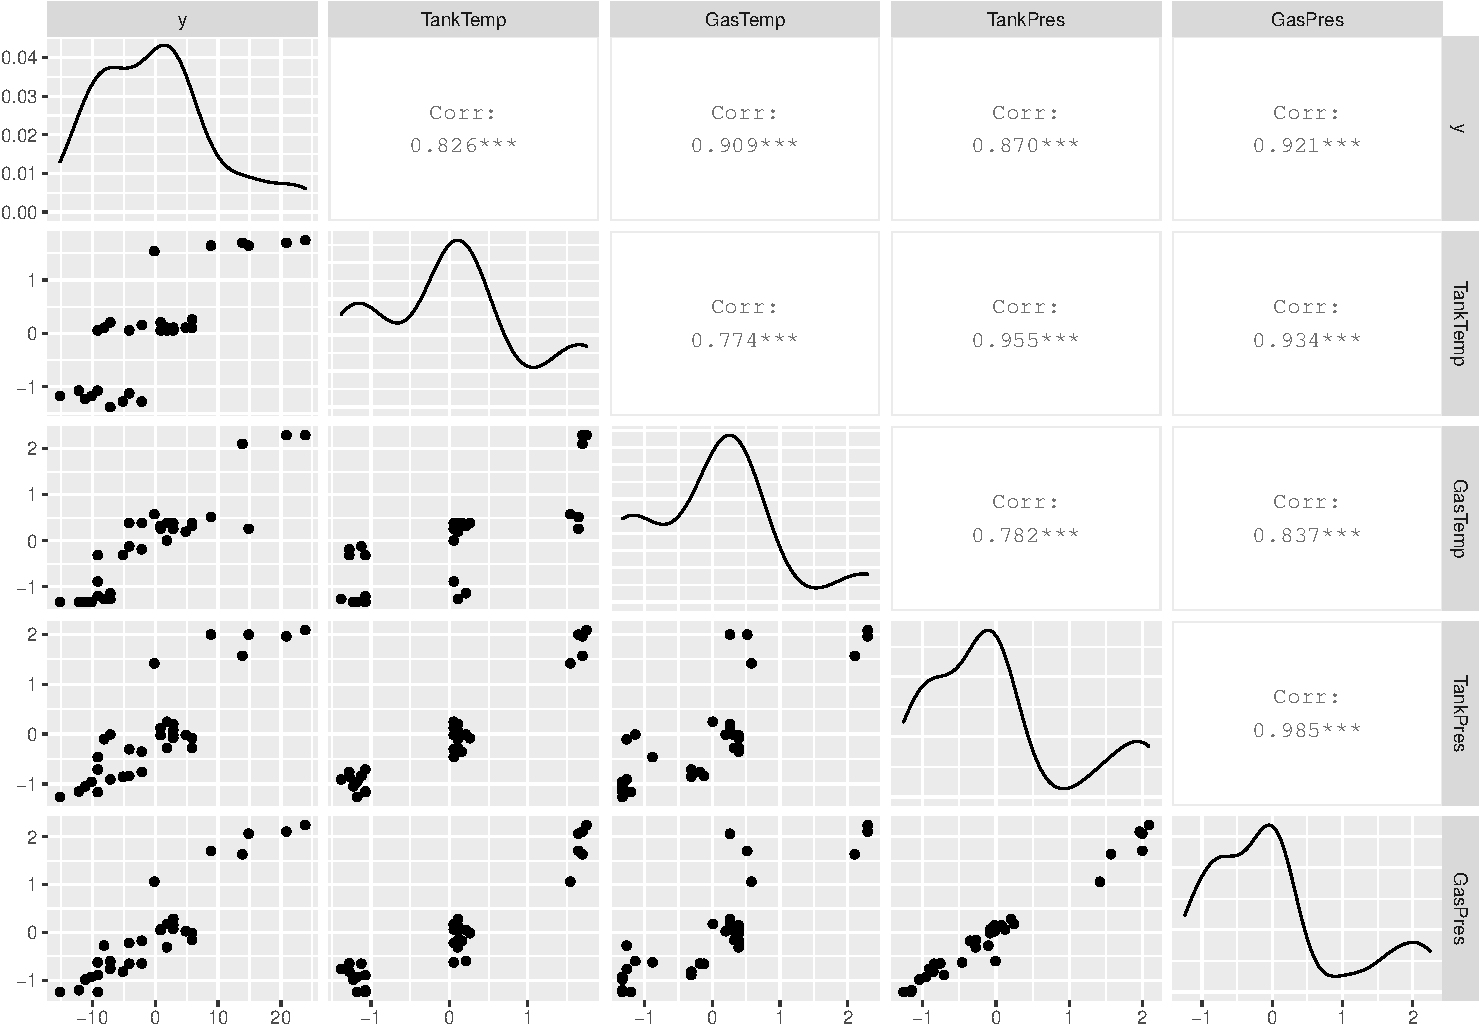
\includegraphics{L2_files/figure-beamer/unnamed-chunk-3-1.pdf}

Calculate the estimated covariance matrix of the standardized
covariates. Do you see a potential problem here?

\begin{Shaded}
\begin{Highlighting}[]
\KeywordTok{cov}\NormalTok{(dss)}
\end{Highlighting}
\end{Shaded}

\begin{verbatim}
##                  y  TankTemp   GasTemp  TankPres   GasPres
## y        87.790323 7.7399536 8.5202970 8.1505120 8.6325694
## TankTemp  7.739954 1.0000000 0.7742909 0.9554116 0.9337690
## GasTemp   8.520297 0.7742909 1.0000000 0.7815286 0.8374639
## TankPres  8.150512 0.9554116 0.7815286 1.0000000 0.9850748
## GasPres   8.632569 0.9337690 0.8374639 0.9850748 1.0000000
\end{verbatim}

\end{frame}

\begin{frame}[fragile]

We have fitted a MLR with all four covariates. Explain what you see.

\begin{Shaded}
\begin{Highlighting}[]
\NormalTok{full <-}\StringTok{ }\KeywordTok{lm}\NormalTok{(y}\OperatorTok{~}\NormalTok{.,dss)}
\KeywordTok{summary}\NormalTok{(full)}
\end{Highlighting}
\end{Shaded}

\begin{verbatim}
## 
## Call:
## lm(formula = y ~ ., data = dss)
## 
## Residuals:
##    Min     1Q Median     3Q    Max 
## -5.586 -1.221 -0.118  1.320  5.106 
## 
## Coefficients:
##               Estimate Std. Error t value Pr(>|t|)   
## (Intercept)  4.851e-15  4.826e-01   0.000  1.00000   
## TankTemp    -5.582e-01  1.768e+00  -0.316  0.75461   
## GasTemp      3.395e+00  1.065e+00   3.187  0.00362 **
## TankPres    -6.274e+00  4.140e+00  -1.515  0.14132   
## GasPres      1.249e+01  3.859e+00   3.237  0.00319 **
## ---
## Signif. codes:  0 '***' 0.001 '**' 0.01 '*' 0.05 '.' 0.1 ' ' 1
## 
## Residual standard error: 2.73 on 27 degrees of freedom
## Multiple R-squared:  0.9261, Adjusted R-squared:  0.9151 
## F-statistic: 84.54 on 4 and 27 DF,  p-value: 7.249e-15
\end{verbatim}

\begin{Shaded}
\begin{Highlighting}[]
\KeywordTok{confint}\NormalTok{(full)}
\end{Highlighting}
\end{Shaded}

\begin{verbatim}
##                   2.5 %     97.5 %
## (Intercept)  -0.9902125  0.9902125
## TankTemp     -4.1852036  3.0688444
## GasTemp       1.2093630  5.5812551
## TankPres    -14.7689131  2.2214176
## GasPres       4.5730466 20.4078380
\end{verbatim}

\begin{Shaded}
\begin{Highlighting}[]
\KeywordTok{ggplot}\NormalTok{(full, }\KeywordTok{aes}\NormalTok{(.fitted, .stdresid)) }\OperatorTok{+}\StringTok{ }\KeywordTok{geom_point}\NormalTok{(}\DataTypeTok{pch =} \DecValTok{21}\NormalTok{) }\OperatorTok{+}\StringTok{ }\KeywordTok{geom_hline}\NormalTok{(}\DataTypeTok{yintercept =} \DecValTok{0}\NormalTok{, }
    \DataTypeTok{linetype =} \StringTok{"dashed"}\NormalTok{) }\OperatorTok{+}\StringTok{ }\KeywordTok{geom_smooth}\NormalTok{(}\DataTypeTok{se =} \OtherTok{FALSE}\NormalTok{, }\DataTypeTok{col =} \StringTok{"red"}\NormalTok{, }\DataTypeTok{size =} \FloatTok{0.5}\NormalTok{, }
    \DataTypeTok{method =} \StringTok{"loess"}\NormalTok{) }\OperatorTok{+}\StringTok{ }\KeywordTok{labs}\NormalTok{(}\DataTypeTok{x =} \StringTok{"Fitted values"}\NormalTok{, }\DataTypeTok{y =} \StringTok{"Standardized residuals"}\NormalTok{, }
    \DataTypeTok{title =} \StringTok{"Fitted values vs standardized residuals"}\NormalTok{, }\DataTypeTok{subtitle =} \KeywordTok{deparse}\NormalTok{(full}\OperatorTok{$}\NormalTok{call))}
\end{Highlighting}
\end{Shaded}

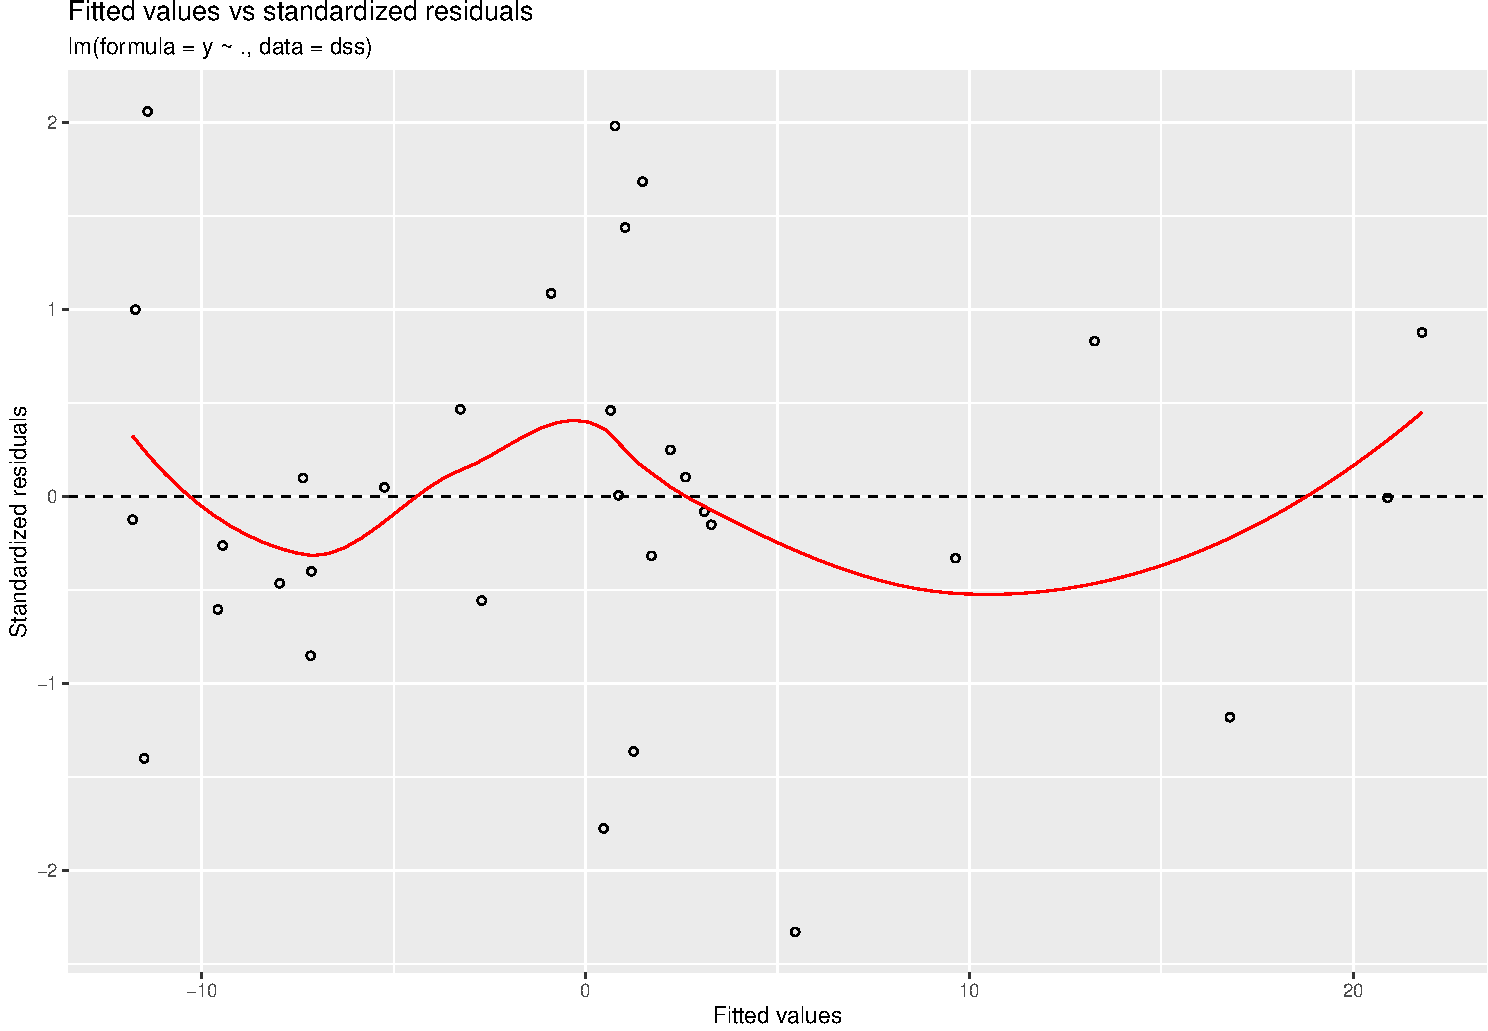
\includegraphics{L2_files/figure-beamer/unnamed-chunk-5-1.pdf}

\begin{Shaded}
\begin{Highlighting}[]
\KeywordTok{ggplot}\NormalTok{(full, }\KeywordTok{aes}\NormalTok{(}\DataTypeTok{sample =}\NormalTok{ .stdresid)) }\OperatorTok{+}\StringTok{ }\KeywordTok{stat_qq}\NormalTok{(}\DataTypeTok{pch =} \DecValTok{19}\NormalTok{) }\OperatorTok{+}\StringTok{ }\KeywordTok{geom_abline}\NormalTok{(}\DataTypeTok{intercept =} \DecValTok{0}\NormalTok{, }
    \DataTypeTok{slope =} \DecValTok{1}\NormalTok{, }\DataTypeTok{linetype =} \StringTok{"dotted"}\NormalTok{) }\OperatorTok{+}\StringTok{ }\KeywordTok{labs}\NormalTok{(}\DataTypeTok{x =} \StringTok{"Theoretical quantiles"}\NormalTok{, }
    \DataTypeTok{y =} \StringTok{"Standardized residuals"}\NormalTok{, }\DataTypeTok{title =} \StringTok{"Normal Q-Q"}\NormalTok{, }\DataTypeTok{subtitle =} \KeywordTok{deparse}\NormalTok{(full}\OperatorTok{$}\NormalTok{call))}
\end{Highlighting}
\end{Shaded}

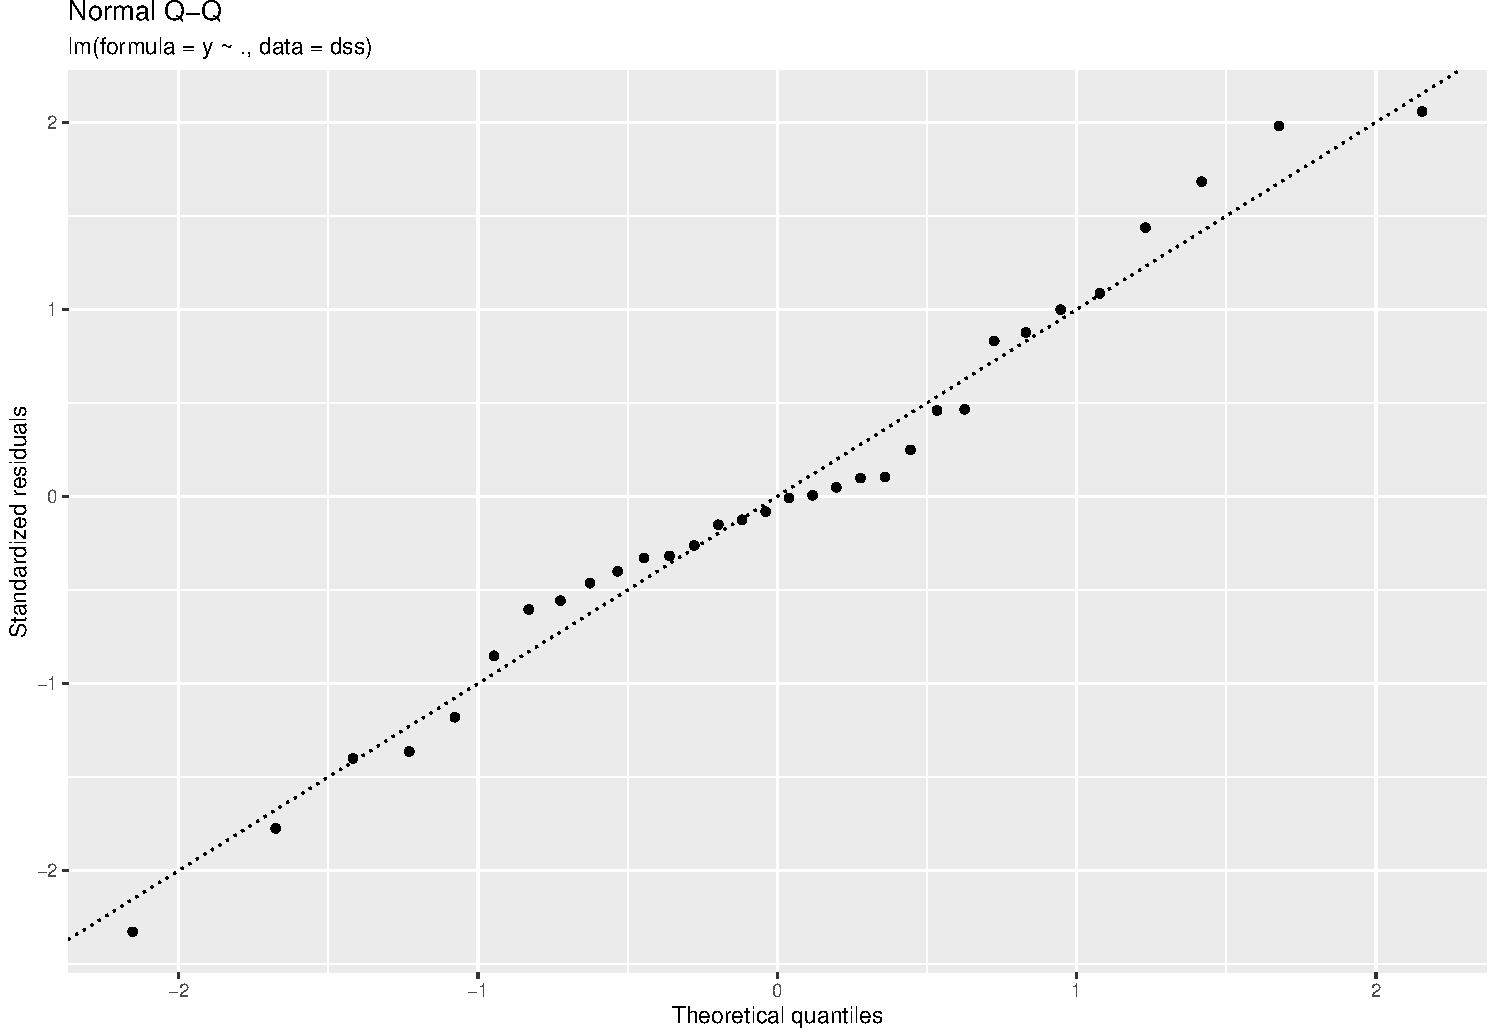
\includegraphics{L2_files/figure-beamer/unnamed-chunk-5-2.pdf}

\begin{Shaded}
\begin{Highlighting}[]
\KeywordTok{ad.test}\NormalTok{(}\KeywordTok{rstudent}\NormalTok{(full))}
\end{Highlighting}
\end{Shaded}

\begin{verbatim}
## 
##  Anderson-Darling normality test
## 
## data:  rstudent(full)
## A = 0.3588, p-value = 0.43
\end{verbatim}

\end{frame}

\begin{frame}[fragile]

Perform best subset selection using Mallows \(C_p\) (equivalent to AIC)
to choose the best model.

\begin{Shaded}
\begin{Highlighting}[]
\NormalTok{bests <-}\StringTok{ }\KeywordTok{regsubsets}\NormalTok{(x,y)}
\NormalTok{sumbests <-}\StringTok{ }\KeywordTok{summary}\NormalTok{(bests)}
\KeywordTok{print}\NormalTok{(sumbests)}
\end{Highlighting}
\end{Shaded}

\begin{verbatim}
## Subset selection object
## 4 Variables  (and intercept)
##          Forced in Forced out
## TankTemp     FALSE      FALSE
## GasTemp      FALSE      FALSE
## TankPres     FALSE      FALSE
## GasPres      FALSE      FALSE
## 1 subsets of each size up to 4
## Selection Algorithm: exhaustive
##          TankTemp GasTemp TankPres GasPres
## 1  ( 1 ) " "      " "     " "      "*"    
## 2  ( 1 ) " "      "*"     " "      "*"    
## 3  ( 1 ) " "      "*"     "*"      "*"    
## 4  ( 1 ) "*"      "*"     "*"      "*"
\end{verbatim}

\begin{Shaded}
\begin{Highlighting}[]
\KeywordTok{which.min}\NormalTok{(sumbests}\OperatorTok{$}\NormalTok{cp) }
\end{Highlighting}
\end{Shaded}

\begin{verbatim}
## [1] 3
\end{verbatim}

\end{frame}

\begin{frame}[fragile]

Model after best subset selection.

\begin{Shaded}
\begin{Highlighting}[]
\NormalTok{red <-}\StringTok{ }\KeywordTok{lm}\NormalTok{(y}\OperatorTok{~}\NormalTok{GasTemp}\OperatorTok{+}\NormalTok{TankPres}\OperatorTok{+}\NormalTok{GasPres,}\DataTypeTok{data=}\NormalTok{dss)}
\KeywordTok{summary}\NormalTok{(red)}
\end{Highlighting}
\end{Shaded}

\begin{verbatim}
## 
## Call:
## lm(formula = y ~ GasTemp + TankPres + GasPres, data = dss)
## 
## Residuals:
##     Min      1Q  Median      3Q     Max 
## -5.6198 -1.2934 -0.0496  1.4858  4.9131 
## 
## Coefficients:
##               Estimate Std. Error t value Pr(>|t|)   
## (Intercept)  5.131e-15  4.748e-01   0.000  1.00000   
## GasTemp      3.290e+00  9.951e-01   3.306  0.00260 **
## TankPres    -7.099e+00  3.159e+00  -2.247  0.03272 * 
## GasPres      1.287e+01  3.607e+00   3.568  0.00132 **
## ---
## Signif. codes:  0 '***' 0.001 '**' 0.01 '*' 0.05 '.' 0.1 ' ' 1
## 
## Residual standard error: 2.686 on 28 degrees of freedom
## Multiple R-squared:  0.9258, Adjusted R-squared:  0.9178 
## F-statistic: 116.4 on 3 and 28 DF,  p-value: 6.427e-16
\end{verbatim}

\begin{Shaded}
\begin{Highlighting}[]
\KeywordTok{confint}\NormalTok{(red)}
\end{Highlighting}
\end{Shaded}

\begin{verbatim}
##                   2.5 %     97.5 %
## (Intercept)  -0.9725378  0.9725378
## GasTemp       1.2513019  5.3281126
## TankPres    -13.5706954 -0.6270544
## GasPres       5.4823283 20.2586338
\end{verbatim}

\end{frame}

\begin{frame}{Ridge regression}
\protect\hypertarget{ridge-regression}{}

(ELS 3.4.1)

Ridge regression is also called ``Tikhonov regularization''.

We consider the classical linear model set-up, as for the LS estimation,
but now we look at shrinking the coefficients towards 0 to construct
biased estimators - and then ``hope'' that this also has made the
variances decrease.

We will not shrink the intercept \(\beta_0\), because then the this will
depend on the origin of the response.

The ridge solution is dependent on the scaling of the covariates, and
usually we work with standardized covariates and also with centered
response.

\end{frame}

\begin{frame}

\begin{block}{Minimization problem}

\begin{block}{Budget version}

We want to constrain the size of the estimated regression parameters, so
we give the sum of squared regression coefficients a budget \(t\).

Minimize the squared error loss

\[ \sum_{i=1}^N (y_i-\beta_0-\sum_{j=1}^p x_{ij}\beta_j )^2 \] subject
to \(\sum_{j=1}^p \beta_j^2 \le t\). The solution is called
\(\hat{\beta}_{\text{ridge}}\).

\end{block}

\end{block}

\end{frame}

\begin{frame}

\begin{figure}
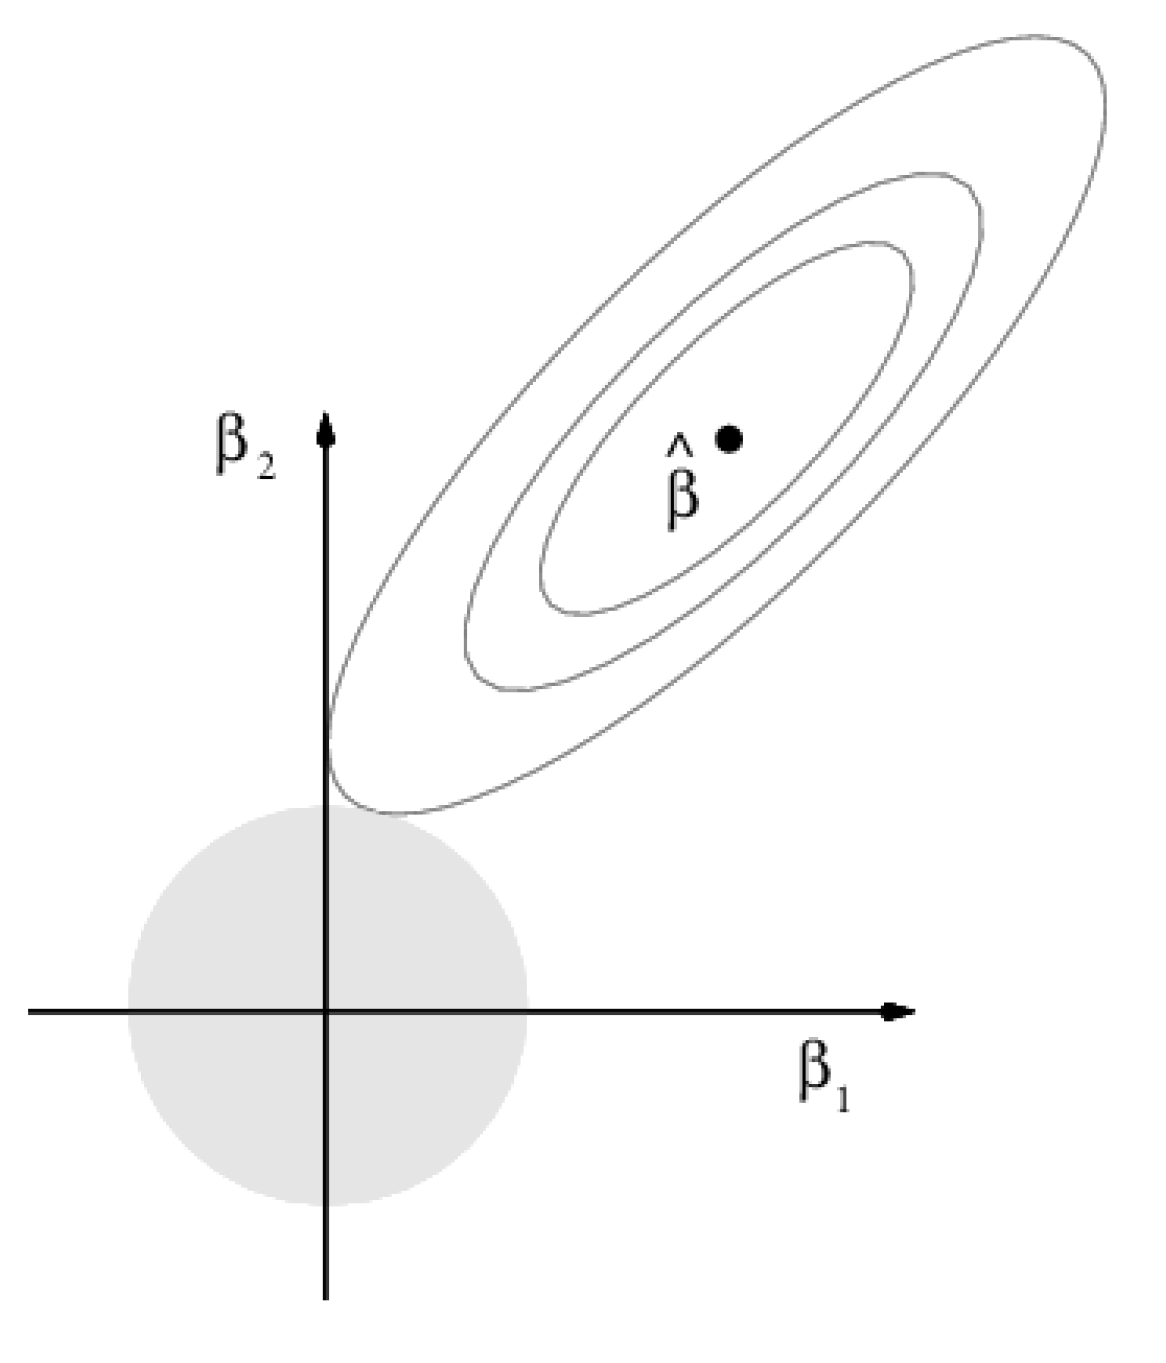
\includegraphics[width=0.4\linewidth]{./ILS67ridge} \caption{Figure from An Introduction to Statistical Learning, with applications in R (Springer, 2013) with permission from the authors: G. James, D. Witten, T. Hastie and R. Tibshirani.}\label{fig:unnamed-chunk-8}
\end{figure}

\end{frame}

\begin{frame}

\begin{block}{Penalty version}

\[ \hat{\beta}_{\text{ridge}}= \text{argmin}_{\beta}[\sum_{i=1}^N (y_i-\beta_0-\sum_{j=1}^p x_{ij}\beta_j )^2 + \lambda \sum_{j=1}^p \beta_j^2]\]
where \(\lambda \le 0\) is a complexity (regularization, penalty)
parameter controlling the amount of shrinkage.

\begin{itemize}
\tightlist
\item
  The larger \(\lambda\) the greater the amount of shrinkage
\item
  The shrinkage is towards 0
\end{itemize}

This version of the problem is also called the Lagrangian form.

The budget and penalty minimization problems are equivalent ways to
write the ridge regression and there is a one-to-one correspondence
between the budget \(t\) and the penalty \(\lambda\).

\end{block}

\end{frame}

\begin{frame}

\begin{block}{Parameter estimation}

As explained, centred covariates and responses are used - and the
intercept term is removed from the model. Then NOW \({\bf X}\) does not
include a column with 1s and has dimension \(N \times p\).

Penalty criterion to minimize

\[ ({\bf y}-{\bf X}\beta)^T ({\bf y}-{\bf X}\beta)+ \lambda \beta^T \beta \]
This can be rewritten as

\[ {\bf y}^T{\bf y}-2{\bf y}^T{\bf X}\beta+\beta^T({\bf X}^T{\bf X}+\lambda {\bf I})\beta\]

\end{block}

\end{frame}

\begin{frame}

Proceeding along the lines as done with the LS estimation, we get the
(new) normal equations

\[ ({\bf X}^T{\bf X}+\lambda {\bf I})\beta= {\bf X}^T {\bf Y}\]

and the estimator:

\[ \hat{\beta}_{\text{ridge}}=({\bf X}^T{\bf X}+\lambda {\bf I})^{-1} {\bf X}^T {\bf Y}\]

\end{frame}

\begin{frame}

Observe that the solution adds a positive constant \(\lambda\) to the
diagonal of \({\bf X}^T{\bf X}\), so that even if \({\bf X}^T{\bf X}\)
does not have full rank then the problem is non-singular and we can
invert \(({\bf X}^T{\bf X}+\lambda {\bf I})\).

When ridge regression was introduced in statistics in the 1970s this
(avoiding non-singuarlity) was the motivation.

When \(N<p\) then the design matrix will have rank less than the number
of covariates, and the LS estimate does not exist.

The case when two or more covariates are perfectly linearly dependent is
called \emph{super-collinearity} (accoring to WNvN).

\end{frame}

\begin{frame}

\end{frame}

\begin{frame}[fragile]

\begin{block}{Gasoline continued}

\begin{Shaded}
\begin{Highlighting}[]
\NormalTok{start=}\KeywordTok{glmnet}\NormalTok{(}\DataTypeTok{x=}\NormalTok{x,}\DataTypeTok{y=}\NormalTok{y,}\DataTypeTok{alpha=}\DecValTok{0}\NormalTok{)}
\NormalTok{autolambda=start}\OperatorTok{$}\NormalTok{lambda }\CommentTok{# automatic choice of lambda had smallest lambda 0.96 - but I added more small values to also be able to see that LS-solution is for lambda=0}
\NormalTok{newlambda=}\KeywordTok{c}\NormalTok{(autolambda,}\FloatTok{0.5}\NormalTok{,}\FloatTok{0.3}\NormalTok{,}\FloatTok{0.2}\NormalTok{,}\FloatTok{0.1}\NormalTok{)}
\NormalTok{fit.ridge=}\KeywordTok{glmnet}\NormalTok{(x,y,}\DataTypeTok{alpha=}\DecValTok{0}\NormalTok{,}\DataTypeTok{lambda=}\NormalTok{newlambda)}
\KeywordTok{plot}\NormalTok{(fit.ridge,}\DataTypeTok{xvar=}\StringTok{"lambda"}\NormalTok{,}\DataTypeTok{label=}\OtherTok{TRUE}\NormalTok{)}
\end{Highlighting}
\end{Shaded}

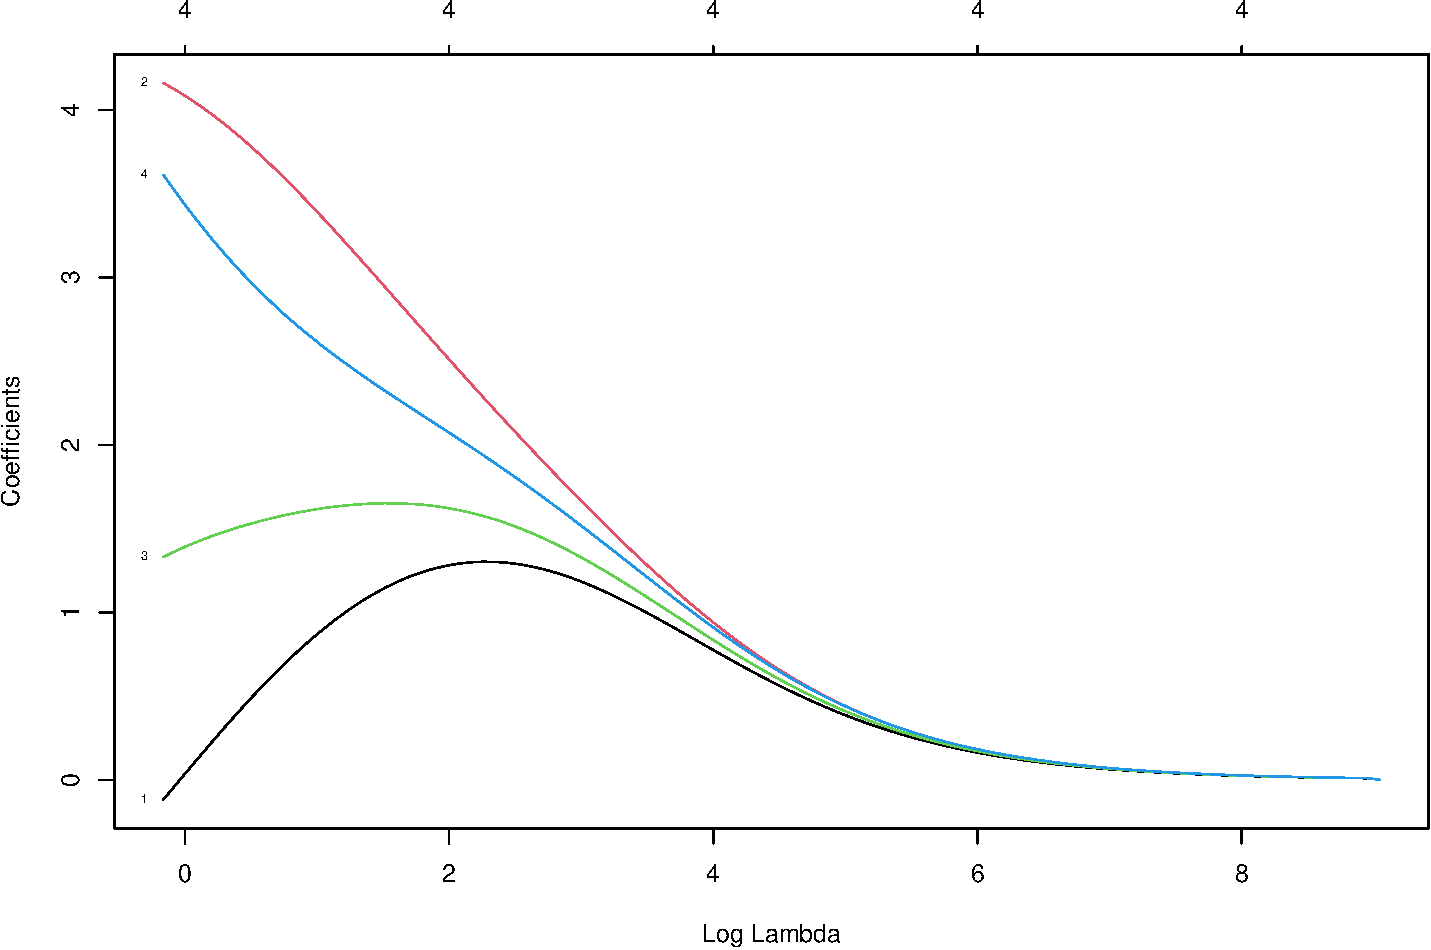
\includegraphics{L2_files/figure-beamer/unnamed-chunk-9-1.pdf}

\begin{Shaded}
\begin{Highlighting}[]
\CommentTok{#plot(fit.ridge,xvar="norm",label=TRUE)}
\end{Highlighting}
\end{Shaded}

\end{block}

\end{frame}

\begin{frame}[fragile]

\begin{block}{Model selection}

To choose the optimal penalty parameter \(\lambda\) cross-validation is
the default method in use. ELS recommends to either

\begin{itemize}
\tightlist
\item
  choose the \(\lambda\) corresponding to the smallest CV error
\item
  or first find the \(\lambda\) with the smallest CV-error, and then
  record the estimated standard error of the CV-error at this value, and
  then choose the largest \(\lambda\) such that the CV error is still
  within one standard error of the minimum. We choose the largest
  because we want the less flexible model.
\end{itemize}

The R package \texttt{glmnet} (by Hastie et al) has default \(K=10\)
fold cross-validation with the function \texttt{cv.glmnet} where
\texttt{alpha=0} gives the ridge penalty.

\end{block}

\end{frame}

\begin{frame}[fragile]

\begin{block}{Gasoline continued}

Explain what you see!

\begin{Shaded}
\begin{Highlighting}[]
\NormalTok{cv.ridge=}\KeywordTok{cv.glmnet}\NormalTok{(x,y,}\DataTypeTok{alpha=}\DecValTok{0}\NormalTok{,}\DataTypeTok{lambda=}\NormalTok{newlambda)}
\KeywordTok{print}\NormalTok{(}\KeywordTok{paste}\NormalTok{(}\StringTok{"The lamda giving the smallest CV error"}\NormalTok{,cv.ridge}\OperatorTok{$}\NormalTok{lambda.min))}
\end{Highlighting}
\end{Shaded}

\begin{verbatim}
## [1] "The lamda giving the smallest CV error 0.1"
\end{verbatim}

\begin{Shaded}
\begin{Highlighting}[]
\KeywordTok{print}\NormalTok{(}\KeywordTok{paste}\NormalTok{(}\StringTok{"The 1sd err method lambda"}\NormalTok{,cv.ridge}\OperatorTok{$}\NormalTok{lambda}\FloatTok{.1}\NormalTok{se))}
\end{Highlighting}
\end{Shaded}

\begin{verbatim}
## [1] "The 1sd err method lambda 3.43009811945866"
\end{verbatim}

\begin{Shaded}
\begin{Highlighting}[]
\KeywordTok{plot}\NormalTok{(cv.ridge)}
\end{Highlighting}
\end{Shaded}

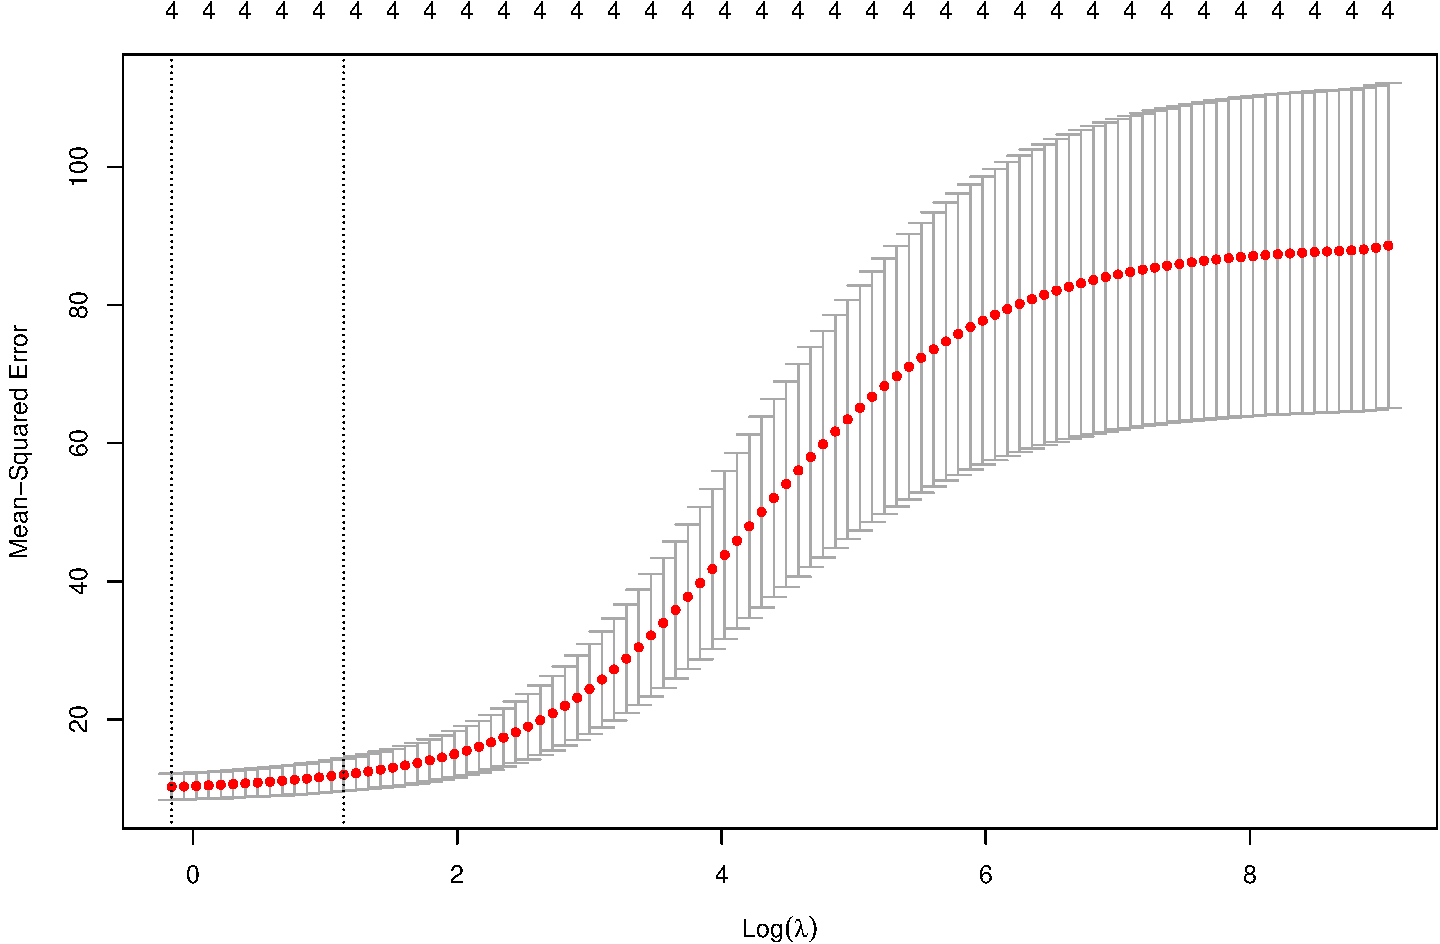
\includegraphics{L2_files/figure-beamer/unnamed-chunk-10-1.pdf}

\begin{Shaded}
\begin{Highlighting}[]
\CommentTok{# use 1sd error rule default}
\KeywordTok{plot}\NormalTok{(fit.ridge,}\DataTypeTok{xvar=}\StringTok{"lambda"}\NormalTok{,}\DataTypeTok{label=}\OtherTok{TRUE}\NormalTok{);}
\KeywordTok{abline}\NormalTok{(}\DataTypeTok{v=}\KeywordTok{log}\NormalTok{(cv.ridge}\OperatorTok{$}\NormalTok{lambda}\FloatTok{.1}\NormalTok{se));}
\end{Highlighting}
\end{Shaded}

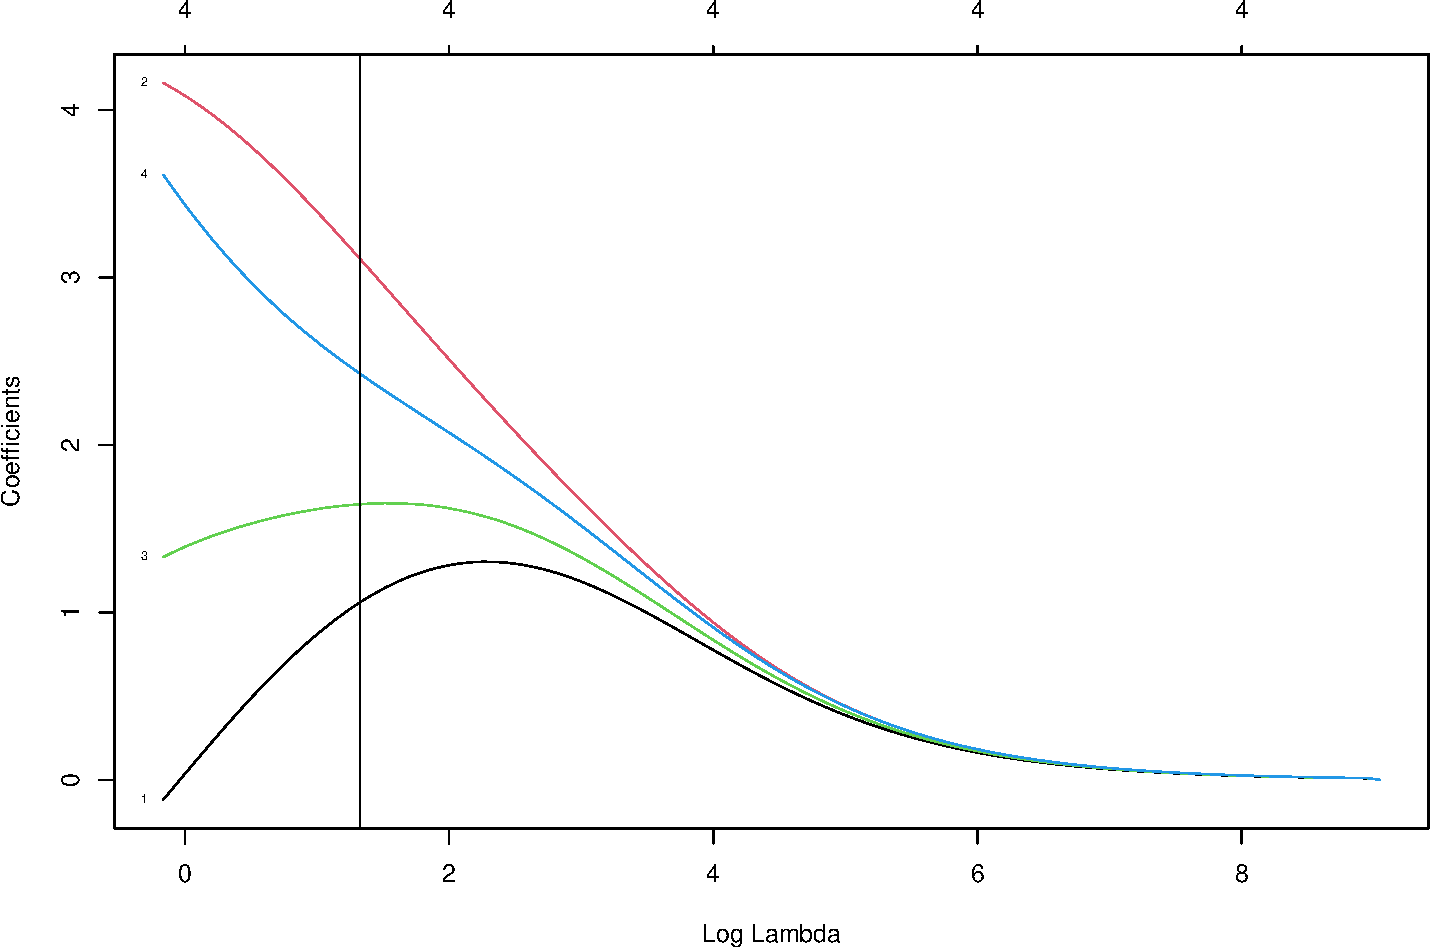
\includegraphics{L2_files/figure-beamer/unnamed-chunk-10-2.pdf}

\begin{Shaded}
\begin{Highlighting}[]
\KeywordTok{coef}\NormalTok{(cv.ridge)}
\end{Highlighting}
\end{Shaded}

\begin{verbatim}
## 5 x 1 sparse Matrix of class "dgCMatrix"
##                        1
## (Intercept) 2.180054e-16
## TankTemp    1.010525e+00
## GasTemp     3.193569e+00
## TankPres    1.639813e+00
## GasPres     2.477606e+00
\end{verbatim}

\begin{Shaded}
\begin{Highlighting}[]
\NormalTok{full}\OperatorTok{$}\NormalTok{coeff}
\end{Highlighting}
\end{Shaded}

\begin{verbatim}
##   (Intercept)      TankTemp       GasTemp      TankPres       GasPres 
##  4.851273e-15 -5.581796e-01  3.395309e+00 -6.273748e+00  1.249044e+01
\end{verbatim}

\begin{Shaded}
\begin{Highlighting}[]
\NormalTok{red}\OperatorTok{$}\NormalTok{coeff}
\end{Highlighting}
\end{Shaded}

\begin{verbatim}
##   (Intercept)       GasTemp      TankPres       GasPres 
##  5.130982e-15  3.289707e+00 -7.098875e+00  1.287048e+01
\end{verbatim}

\end{block}

\end{frame}

\begin{frame}

\begin{block}{Properties of the ridge estimator}

\begin{block}{Mean}

Derive the mean of the ridge estimator.

What happens if:

\begin{itemize}
\tightlist
\item
  \(\lambda \rightarrow 0\)
\item
  \(\lambda \rightarrow \infty\)
\end{itemize}

\href{https://www.math.ntnu.no/emner/TMA4268/Exam/V2019e.pdf}{Exam
problem 12 (TMA4268, 2019)} with
\href{https://www.math.ntnu.no/emner/TMA4268/Exam/e2019sol.html}{solutions}
Alternatively: \href{https://arxiv.org/pdf/1509.09169.pdf}{Wessel N. van
Wieringen: Lecture notes on ridge regression, section 1.4}

\end{block}

\end{block}

\end{frame}

\begin{frame}

\begin{block}{Covariance}

Derive the covariance of the ridge estimator.

What happens if:

\begin{itemize}
\tightlist
\item
  \(\lambda \rightarrow 0\)
\item
  \(\lambda \rightarrow \infty\)
\end{itemize}

(in our centered model without intercept)

Same resources as above.

\end{block}

\end{frame}

\begin{frame}

\begin{block}{Distribution}

For the normal linear model

\[\hat{\beta}(\lambda)_{\text{ridge}} \sim N \{ (\mathbf{X}^T \mathbf{X} + \lambda \mathbf{I}_{p})^{-1} \mathbf{X}^T \mathbf{X} \, \beta,\]
\[\sigma^2 ( \mathbf{X}^T \mathbf{X} + \lambda \mathbf{I}_{p} )^{-1}  \mathbf{X}^T \mathbf{X} ( \mathbf{X}^T \mathbf{X} + \lambda \mathbf{I}_{p} )^{-1}  \}.
\]

\end{block}

\end{frame}

\begin{frame}

\begin{block}{Is ridge ``better than'' LS?}

\begin{itemize}
\item
  We may prove that the variance of the ridge estimator is smaller or
  equal the variance of the LS estimator. See exercise ``Variance of
  ridge compared to LS'', where we need to look at differences of
  covariance matrices and check for positive semi-definite matrix.
\item
  In addition it is possible to prove that given a suitable choice for
  \(\lambda\) the ridge regression estimator may outperform the LS
  estimator in terms of the MSE. See WNvW Section 1.4.3 for the full
  derivation.
\item
  The optimal choice of \(\lambda\) depends both the true regression
  parameters and the error variance. This means that the penalty
  parameter should be chosen in a \emph{data-driven} fashion.
\end{itemize}

\end{block}

\end{frame}

\begin{frame}

\begin{block}{Insight based on SVD}

\begin{block}{Singular value decomposition (SVD)}

Let \({\bf X}\) be a \(N \times p\) matrix.

SVD is a decomposition of a matrix \({\bf X}\) into a product of three
matrices \[{\bf X}={\bf U}{\bf D}{\bf V}^T.\] \({\bf D}\) is an
\((N \times p)\)-dimensional block matrix. Its upper left block is a
\((\mbox{rank}(\mathbf{X}) \times \mbox{rank}(\mathbf{X}))\)-dimensional
digonal matrix with the singular values on the diagonal. The remaining
blocks, zero if \(p=N\). The singular values are equal
\(\sqrt{\mathrm{eigenvalues}({\bf X}{\bf X}^T})=\sqrt{\mathrm{eigenvalues}({\bf X}^T{\bf X})}\).

\(\mathbf{U}\) is an \((n \times n)\)-dimensional matrix with columns
containing the left singular vectors (denoted \(\mathbf{u}_i\)), that
is, the eigenvectors of \({\bf X}{\bf X}^T\)

\(\mathbf{V}\) is a \((p \times p)\)-dimensional matrix with columns
containing the right singular vectors (denoted \(\mathbf{v}_i\)), that
is, the eigenvectors of \({\bf X}^T{\bf X}\).

The columns of \(\mathbf{U}\) and \(\mathbf{V}\) are orthogonal:
\(\mathbf{U}^{\top} \mathbf{U} = \mathbf{I}_{N} = \mathbf{U}\mathbf{U}^T\)
and
\(\mathbf{V}^T \mathbf{V}= \mathbf{I}_{p} = \mathbf{V}\mathbf{V}^T\).

\end{block}

\end{block}

\end{frame}

\begin{frame}

Following the derivation of WNvW page 11-12:

\begin{itemize}
\tightlist
\item
  If \(n>p\) and the rank of \({\bf X}\) is \(p\), then the LS estimator
  \(\hat{\beta}_{\text{LS}}\) can be written
\end{itemize}

\[\hat{\beta}_{\text{LS}}= \mathbf{V}(\mathbf{D}^T \mathbf{D})^{-1} \mathbf{D}^T \mathbf{U}^T \mathbf{Y}\]

\begin{itemize}
\tightlist
\item
  The ridge estimator \(\hat{\beta}_{\text{ridge}}\)
\end{itemize}

\[ \hat{\beta}_{\text{ridge}}=\mathbf{V} (\mathbf{D}^T \mathbf{D} + \lambda \mathbf{I})^{-1}  \mathbf{D}^T \mathbf{U}^T \mathbf{Y}\]

\begin{itemize}
\tightlist
\item
  The principal component regression based on the first \(k\) principal
  components
\end{itemize}

\[ \hat{\beta}_{\text{PCR}} = \mathbf{V}_{k} (\mathbf{I}_{kp} \mathbf{D}^T \mathbf{D}\mathbf{I}_{pk})^{-1} \mathbf{I}_{kp} \mathbf{D}^T \mathbf{U}^T \mathbf{Y}\]

here \(\mathbf{V}_{k}\) contains the first \(k\) right singular vectors
as columns, and \({\bf I}_{kp}\) is obtained by \({\bf I}_p\) by
removing the last \(p-k\) columns.

\end{frame}

\begin{frame}

Connection to principal component analysis: The estimated covariance
matrix for centred covariates is \(\frac{1}{N}{\bf X}^T{\bf X}\). The
eigenvalues of \({\bf X}^T{\bf X}\) are the squared singular values,
\(d^2_j\). The small singular values \(d_j\) correspond to directions in
the column space of \({\bf X}\) with small variance, which will be the
direction for the last principal components.

The ridge penalties shrinks the direction with the small singular values
the most. Principal components thresholds coefficients in the direction
with singular values of \({\bf X}\), while ridge regression shrinks the
coefficients in these directions.

\end{frame}

\begin{frame}

Alternatively, it is possible to consider the prediction

\[\hat{y}_{\text{LS}}={\bf X}\hat{\beta}_{\text LS}= \cdots = {\bf U}{\bf U}^T {\bf y}\]

\[\hat{y}_{\text{ridge}}={\bf X}\hat{\beta}_{\text ridge}= \cdots =
{\bf U}{\bf D}^2({\bf D}^2+\lambda {\bf I}_p)^{-1}{\bf U}^T {\bf y}=
\sum_{j=1}^p {\bf u}_j \frac{d_j^2}{d_j^2+\lambda}{\bf u}_j^T {\bf y}\]

\textbf{Group discussion:} What can we conclude from this about what the
\(\lambda\) does with each covariate direction?

\end{frame}

\begin{frame}

\begin{block}{The effective degrees of freedom}

In ELS Ch 7.6 we defined the effective number of parameters (here now
referred to as the \emph{effective degrees of freedom}) for a linear
smoother \(\hat{\bf y}={\bf Sy}\) as

\[\text{df}({\bf S})=\text{trace}({\bf S})\]

For ridge regression our linear smoother is
\[{\bf H}_{\lambda}={\bf X}({\bf X}^T{\bf X}+ \lambda {\bf I})^{-1}{\bf X}^T\]

\end{block}

\end{frame}

\begin{frame}

\(\text{df}(\lambda)=\text{tr}({\bf H}_{\lambda})=\text{tr}({\bf X}({\bf X}^T{\bf X}+ \lambda {\bf I})^{-1}{\bf X}^T)=\cdots=\sum_{j=1}^p \frac{d_j^2}{d_j^2+\lambda}\)

\begin{itemize}
\tightlist
\item
  \(\lambda=0\) gives \(\text{df}(\lambda)=p\)
\item
  \(\lambda \rightarrow \infty\) gives
  \(\text{df}(\lambda)\rightarrow 0\)
\end{itemize}

The \(\text{df}(\lambda)\) is sometimes plotted instead of \(\lambda\)
on the horisontal axis when model complexity is chosen.

\end{frame}

\begin{frame}

\begin{block}{Finally}

\begin{itemize}
\tightlist
\item
  When is ridge preferred to LS? When the LS estimates have high
  variance and many predictors are truly non-zero.
\item
  Ridge is computationally fast.
\item
  Ridge is not very easy to interpret, because all \(p\) predictor are
  included in the final model.
\end{itemize}

\end{block}

\end{frame}

\begin{frame}{Lasso}
\protect\hypertarget{lasso}{}

(ELS 3.4.2)

Now we will do what looks at first sight as a small change - we will use
a budget on the absolute value insted of squared value - moving from the
\(L_2\) to the \(L_1\) norm. But, this will have a large impact on the
parameter estimates - both shrinking - and performing model selection
(by shrinking all the way down to 0).

Again, we will not shrink the intercept \(\beta_0\), because then the
this will depend on the origin of the response, and we will work with
standardized covariates and centered response.

\end{frame}

\begin{frame}

\begin{block}{Minimization problem}

\begin{block}{Budget version}

We want to constrain the size of the estimated regression parameters, so
we give the sum of squared regression coefficients a budget \(t\).

Minimize the squared error loss

\[ \sum_{i=1}^N (y_i-\beta_0-\sum_{j=1}^p x_{ij}\beta_j )^2 \] subject
to \(\sum_{j=1}^p \lvert \beta_j\rvert \le t\). The solution is called
\(\hat{\beta}_{\text{lasso}}\).

\end{block}

\end{block}

\end{frame}

\begin{frame}

\begin{figure}
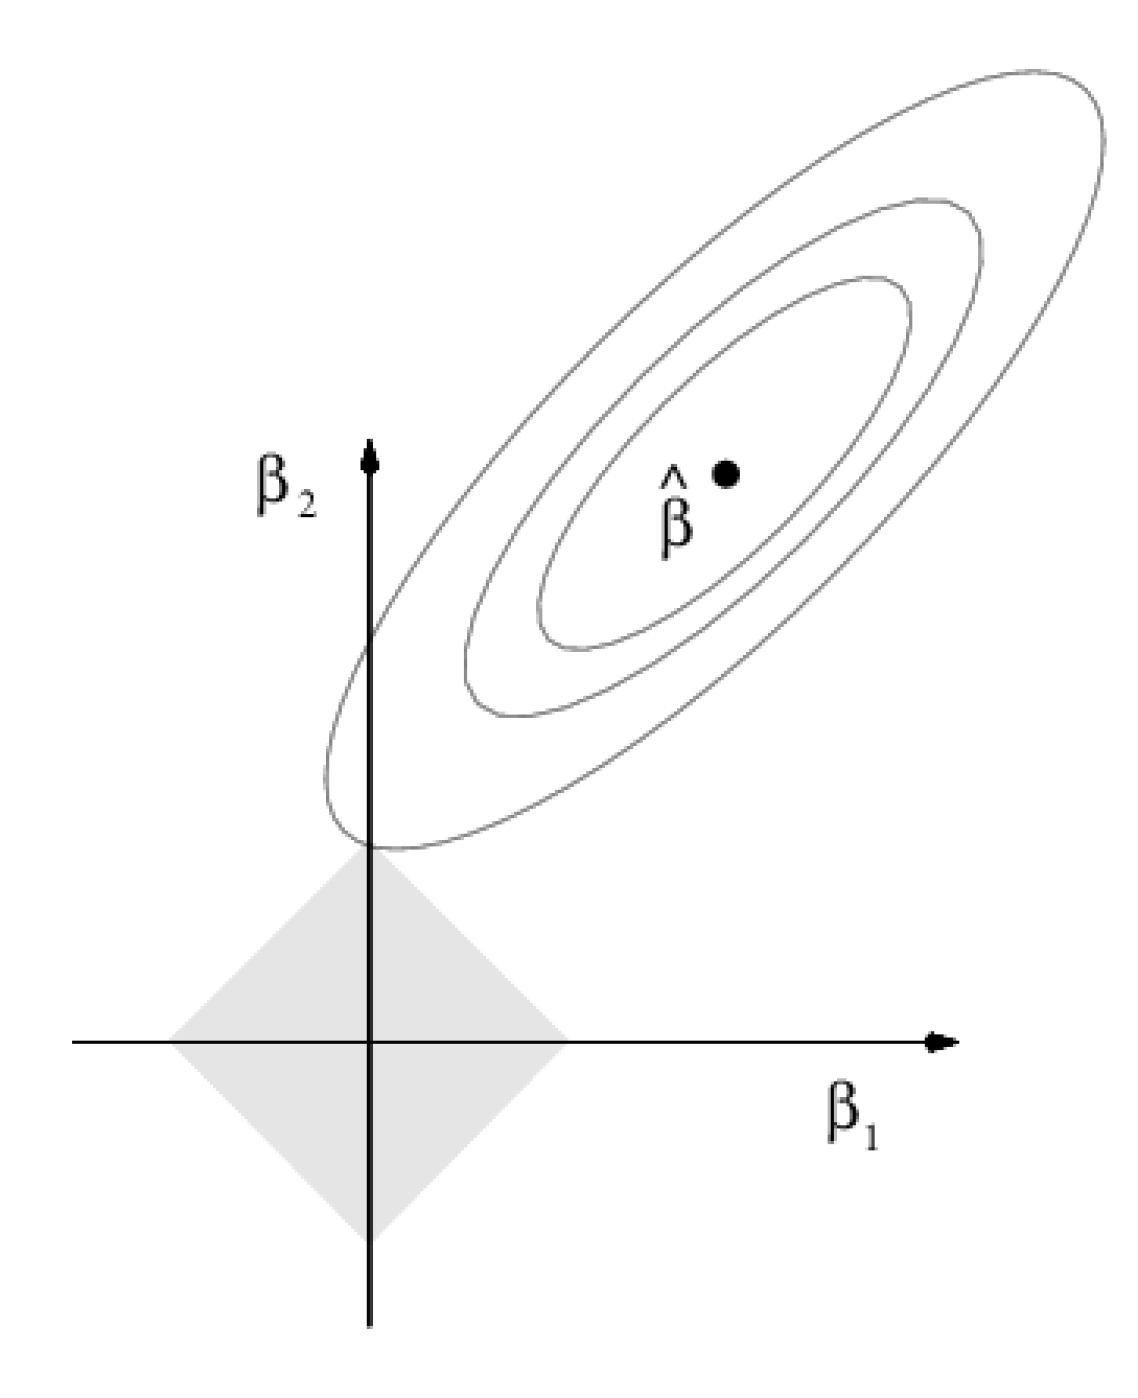
\includegraphics[width=0.5\linewidth]{./ILS67lasso} \caption{Figure from An Introduction to Statistical Learning, with applications in R (Springer, 2013) with permission from the authors: G. James, D. Witten, T. Hastie and R. Tibshirani.}\label{fig:unnamed-chunk-11}
\end{figure}

\end{frame}

\begin{frame}

\begin{block}{Penalty version}

\[ \hat{\beta}_{\text{lasso}}= \text{argmin}_{\beta} [\sum_{i=1}^N (y_i-\beta_0-\sum_{j=1}^p x_{ij}\beta_j )^2 + \lambda \sum_{j=1}^p \lvert \beta_j\rvert ] \]
again, \(\lambda \le 0\) is a complexity (regularization, penalty)
parameter controlling the amount of shrinkage.

\begin{itemize}
\tightlist
\item
  The larger \(\lambda\) the greater the amount of shrinkage
\item
  The shrinkage is towards 0
\end{itemize}

This version of the problem is also called the Lagrangian form.

The budget and penalty minimization problems are equivalent ways to
write the ridge regression and there is a one-to-one correspondence
between the budget \(t\) and the penalty \(\lambda\).

\end{block}

\end{frame}

\begin{frame}

\begin{block}{Small notational difference in the two textbooks}

In HTW an extra \(\frac{1}{2N}\) factor is added to the squared error
for the ridge and the lasso, which is just for ease of interpretation of
a future shrinkage parameter to be included (to make that shrinkage
parameter comparable across different sample sizes in the use of
cross-validation). The factor does not influence the solution of the
minimization of the squared-error loss we consider now.

\end{block}

\end{frame}

\begin{frame}

\begin{block}{Parameter estimation}

\begin{itemize}
\item
  As explained, centred covariates and responses are used - and the
  intercept term is removed from the model. Then \({\bf X}\) does not
  include a column with 1s and has dimension \(N \times p\).
\item
  The use of the absolute value in the penalty term makes the solution
  in general non-linear in \(y_i\), and no closed form solution.
\item
  If we make the budget \(t\) sufficiently small some of the
  coefficients will be exactly zero.
\item
  If \(t\) is chosen larger than
  \(t_0=\sum_{j=1}^p \lvert \hat{\beta}_{{\text {LS}},j} \rvert\) the
  lasso estimates equal the LS estimates.
\item
  The nature of the shrinkage is complex, and will be studied later.
\end{itemize}

In L3 we will look into estimation algorithms for the lasso.

\end{block}

\end{frame}

\begin{frame}

\begin{block}{Conditions for a solution to the penalty version}

(HTW page 9)

The details are found in HTW Chapter 5 (not on our reading list), but
the student familiar with convex analysis, dual problems and
Karush-Kuhn-Tucker (KKT) conditions might find Chapter 5 of interest.

Convex analysis theory: necessary and sufficient conditions for a
solution to the lasso penalty problem is

\[ \frac{1}{N}\langle {\bf x}_j,{\bf y}-{\bf X}\beta \rangle+\lambda s_j=0 \mbox{ for } j=1,\ldots,p\]

where \(\langle a,b \rangle=a^T b\) denotes the inner product. Each
\(s_j\) is an unknow quantity, equal to

\begin{itemize}
\tightlist
\item
  \(\text{sign}(\beta_j)\) if \(\beta_j\neq 0\)
\item
  some value in \([-1,1]\) otherwise (socalled \emph{subgradient} of the
  absolute value function).
\end{itemize}

We may solve this problem in \((\hat{\beta},\hat{s})\), instead of the
penalty version.

\end{block}

\end{frame}

\begin{frame}

\begin{block}{Orthogonal covarates}

This case - explicit solution! New word: soft thresholding".

\end{block}

\end{frame}

\begin{frame}

\begin{figure}
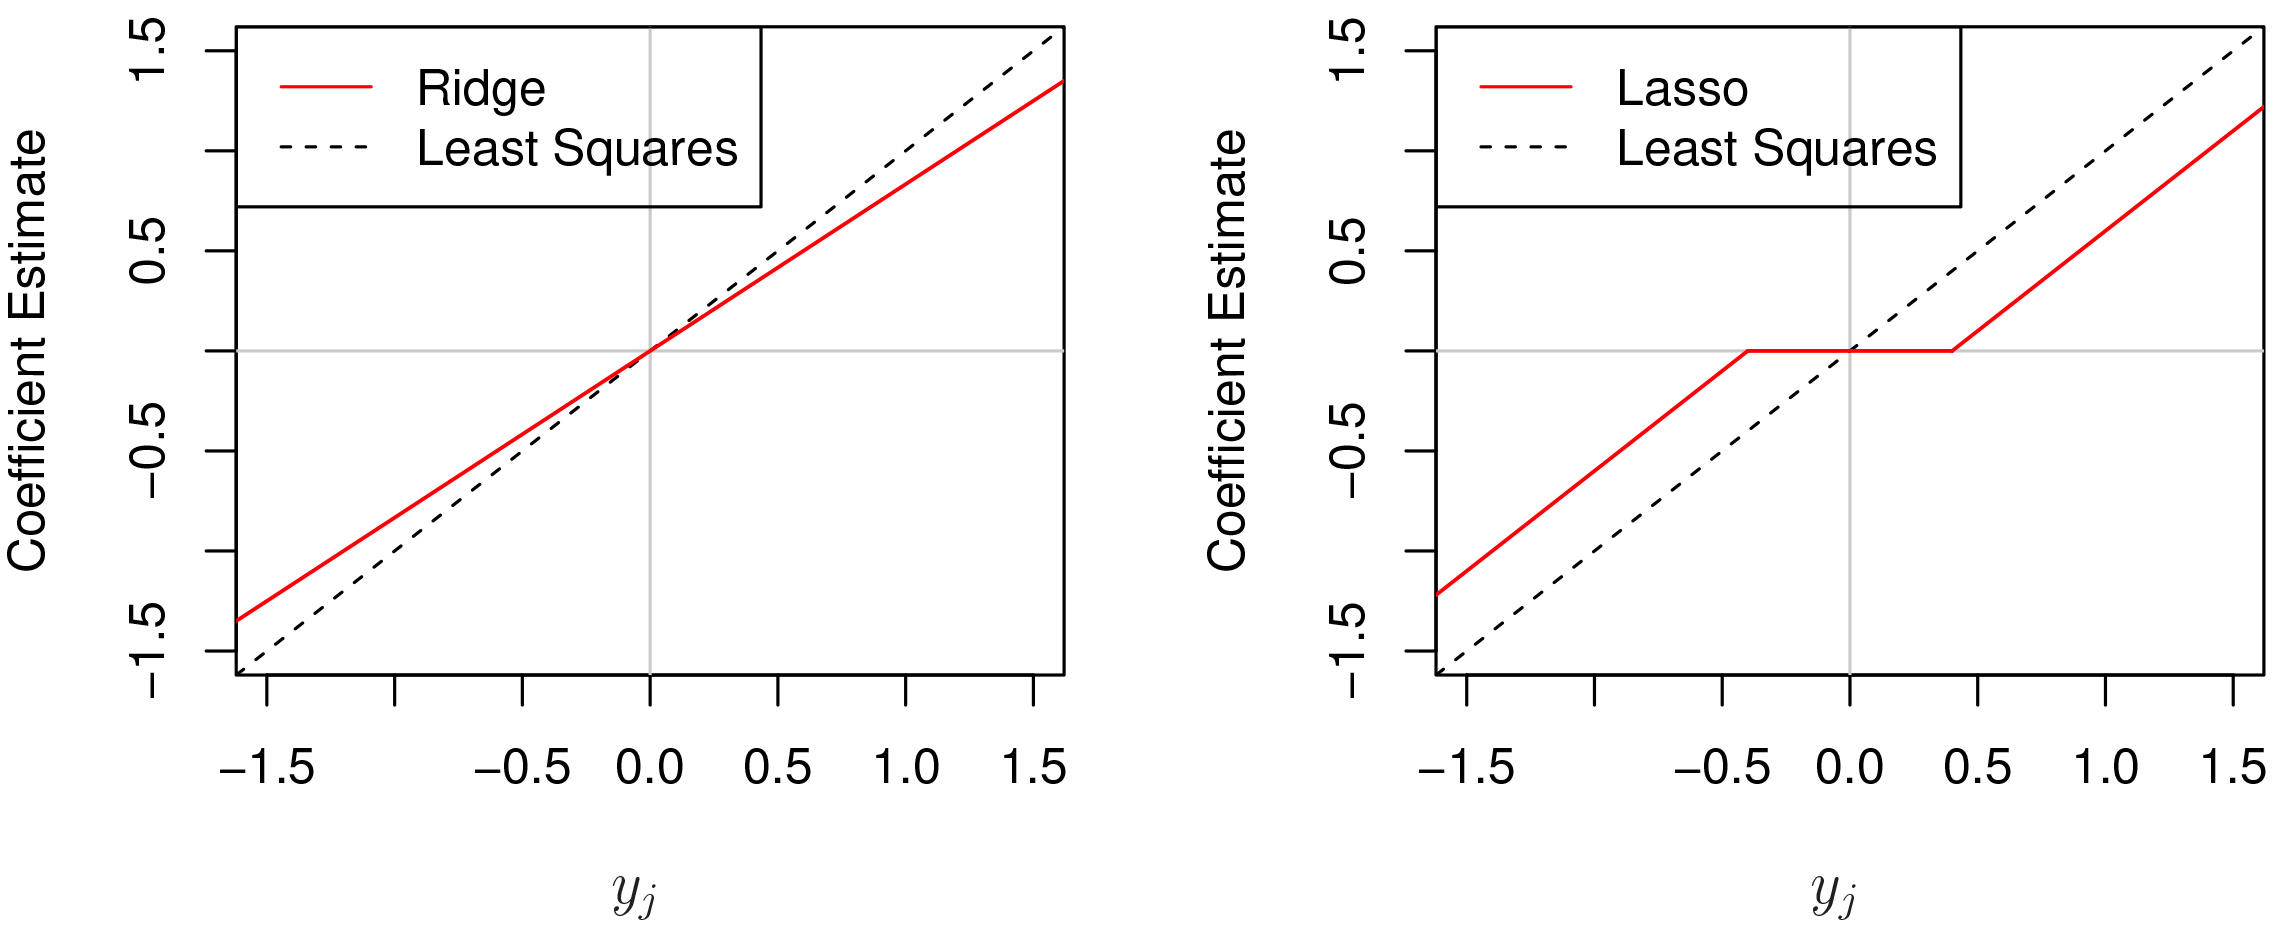
\includegraphics[width=0.5\linewidth]{./ILS610} \caption{Figure from An Introduction to Statistical Learning, with applications in R (Springer, 2013) with permission from the authors: G. James, D. Witten, T. Hastie and R. Tibshirani.}\label{fig:unnamed-chunk-12}
\end{figure}

\end{frame}

\begin{frame}[fragile]

\begin{block}{Gasoline continued}

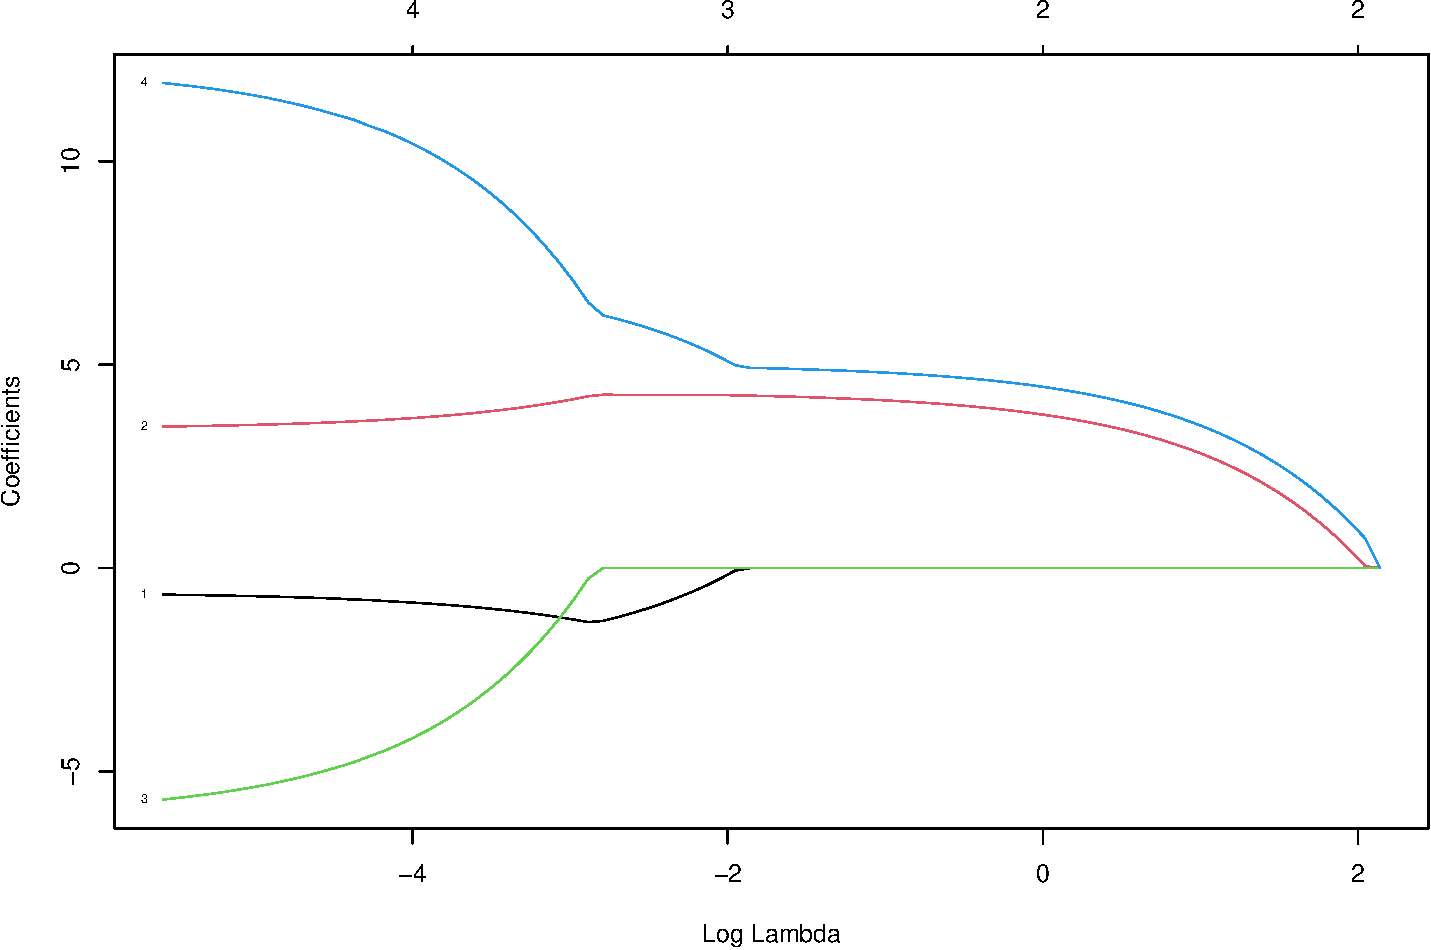
\includegraphics{L2_files/figure-beamer/unnamed-chunk-13-1.pdf}
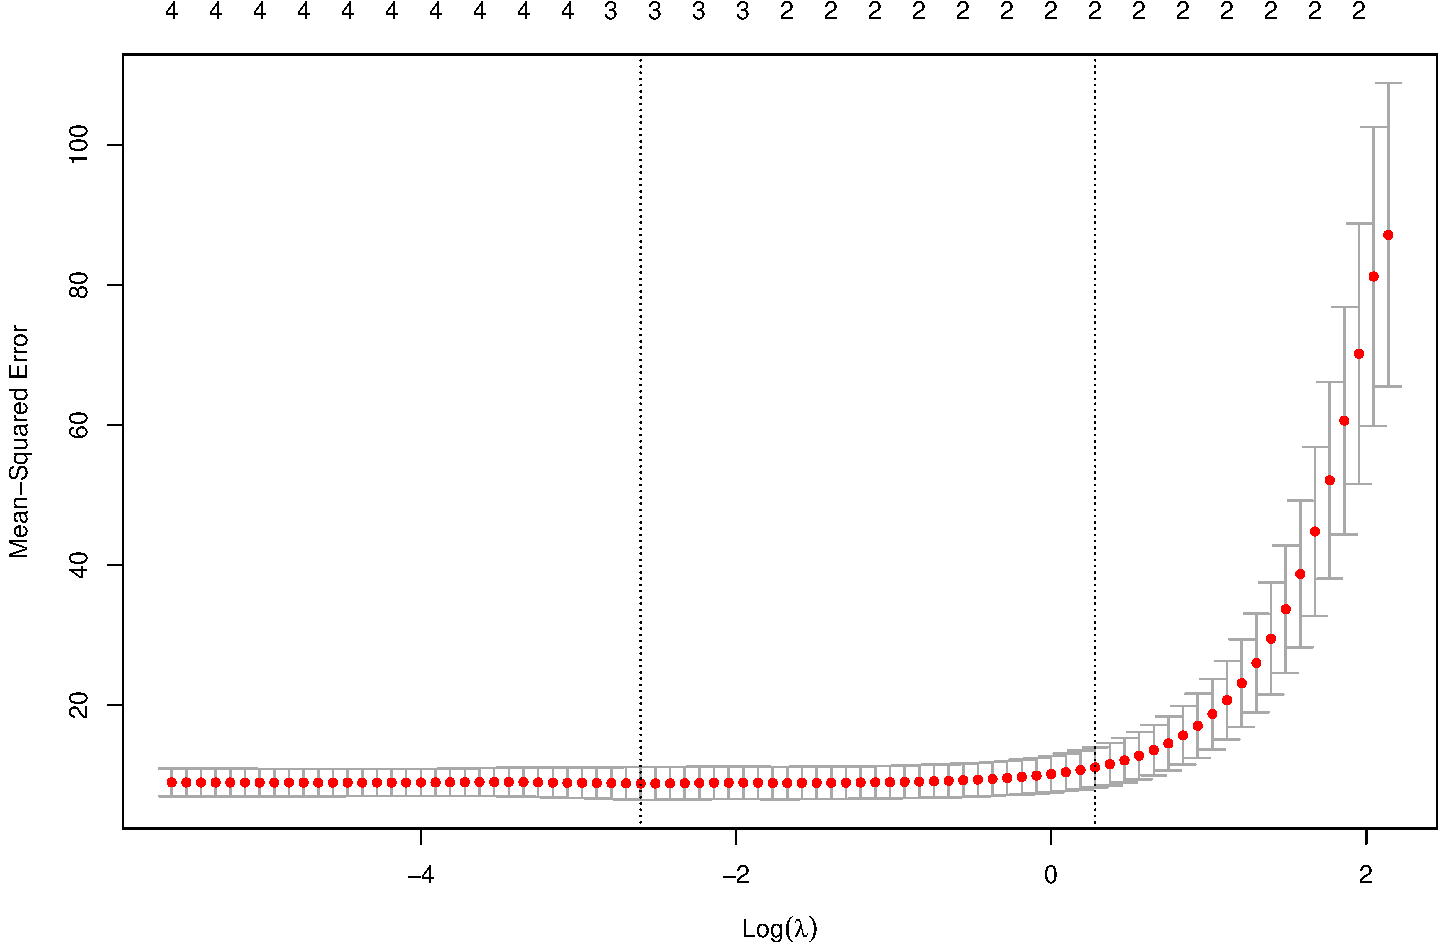
\includegraphics{L2_files/figure-beamer/unnamed-chunk-13-2.pdf}
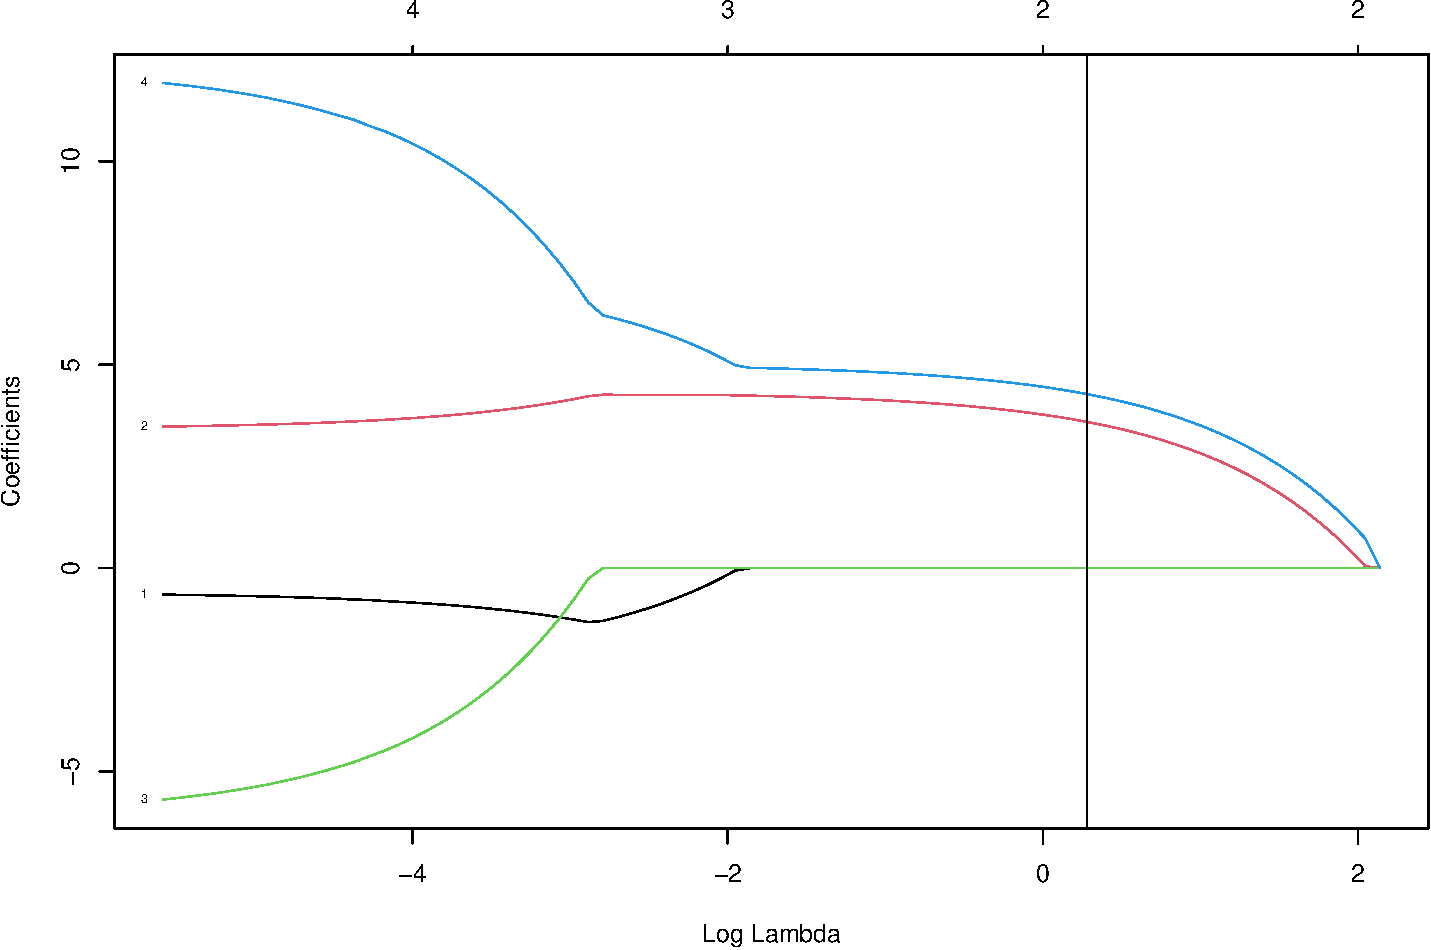
\includegraphics{L2_files/figure-beamer/unnamed-chunk-13-3.pdf}

\begin{verbatim}
## 5 x 1 sparse Matrix of class "dgCMatrix"
##                        1
## (Intercept) 1.028493e-15
## TankTemp    .           
## GasTemp     3.594950e+00
## TankPres    .           
## GasPres     4.278981e+00
\end{verbatim}

\end{block}

\end{frame}

\begin{frame}

\begin{block}{Degrees of freedom}

(HTW 2.5)

In ELS Ch 7.6 we defined the effective number of parameters (here now
referred to as the \emph{effective degrees of freedom}) for a linear
smoother, and used that for the ridge regression. However, the lasso is
not a linear smoother (it is nonlinear in the reponses \(y_i\)).

The lasso is an adaptive fitting procedure, and if our final model has
\(k\) covariates that is different from zero, we would not think that
the effective degrees of freedom for the lasso is then \(k\). However,
it turns out that it is correct to \emph{count} the number of degrees of
freedom by the number of nonzero coefficients.

In ELS Ch 7.6 we also defined the degrees of freedom using the
covariance generalization:
\[\text{df}(\hat{{\bf y}})=\frac{\sum_{i=1}^N \text{Cov}(\hat{y}_i,y_i)}{\sigma_{\varepsilon}^2}\]

where the covariance is taken over the reponse variables, while the
covariates are kept fixed (this formula was developed in connection to
the in-sample prediction error).

\end{block}

\end{frame}

\begin{frame}

It has been shown (HTW refer to this at "somewhat miraculously) that
with a fixed penalty parameter \(\lambda\) the number of non-zero
coefficients \(k_{\lambda}\) is an \emph{unbiased estimate} for the
degrees of freedom.

This is explained by considering that the lasso does not only select
predictors (selecting predictors will give an inflated degrees of
freedom) - but also shrinks the coefficients relative to the LS
estimates. These two forces kind of cancel out.

HTW (page 19): a general proof is difficult, but for an orthogonal
design using the fact that the lasso estimates are soft-thresholded
versions f the univariate regression coefficients for the othogonal
design.

\end{frame}

\begin{frame}

\begin{block}{Finally}

\begin{itemize}
\tightlist
\item
  When is ridge preferred to LS? When the LS estimates have high
  variance and many predictors are truly non-zero.
\item
  Ridge is computationally fast.
\item
  Ridge is not very easy to interpret, because all \(p\) predictor are
  included in the final model.
\end{itemize}

Neigher ridge or lasso dominates the other in all situations.

\end{block}

\end{frame}

\begin{frame}[fragile]{Software}
\protect\hypertarget{software}{}


\includegraphics{logo.png}

We will use the \texttt{glmnet} implementation for R:

\begin{itemize}
\tightlist
\item
  \href{https://cran.r-project.org/web/packages/glmnet/index.html}{R
  glmnet on CRAN} with
  \href{http://www.stanford.edu/~hastie/glmnet}{resources}.

  \begin{itemize}
  \tightlist
  \item
    \href{https://glmnet.stanford.edu/articles/glmnet.html}{Getting
    started}
  \item
    \href{https://glmnet.stanford.edu/articles/glmnetFamily.html}{GLM
    with glmnet}
  \end{itemize}
\end{itemize}

For Python there are different options.

\begin{itemize}
\tightlist
\item
  \href{https://web.stanford.edu/~hastie/glmnet_python/}{Python glmnet}
  is recommended by Hastie et al.
\item
  \href{https://scikit-learn.org/stable/modules/linear_model.html\#ridge-regression-and-classification}{scikit-learn}
  (seems to mostly be for regression? is there lasso for classification
  here?)
\end{itemize}

\end{frame}

\begin{frame}{Exercises}
\protect\hypertarget{exercises}{}

\begin{block}{Gauss-Markov theorem}

The LS is unbiased with the smallest variance among linear predictors:
ELS exercise 3.3a

\end{block}

\begin{block}{Variance of ridge compared to LS}

Consider a classical linear model with regression parameters \(\beta\).
Let \(\hat{\beta}\) be the LS estimator for \(\beta\) and let
\(\tilde{\beta}\) be the ridge regression estimator for \(\beta\). Show
that \(\text{Var}(\hat{\beta}) \ge \text{Var}(\tilde{\beta})\).

\end{block}

\end{frame}

\begin{frame}

\begin{block}{Ridge regression}

This problem is taken, with permission from Wessel van Wieringen, from a
course in High-dimensional data analysis at Vrije University of
Amsterdam.

\begin{block}{a)}

Find the ridge regression solution for the data below for a general
value of \(\lambda\) and for the simple linear regression model
\(Y = \beta_0 + \beta_1 X + \varepsilon\) (only apply the ridge penalty
to the slope parameter, not to the intercept). Show that when
\(\lambda\) is chosen as 40, the ridge solution fit is
\(\hat{Y} = 40 + 1.75 X\).

Data:
\(\mathbf{X}^T = (X_1, X_2, \ldots, X_{8})^T = (-2, -1, -1, -1, 0, 1, 2, 2)^T\),
and
\(\mathbf{Y}^T = (Y_1, Y_2, \ldots, Y_{8})^T = (35, 40, 36, 38, 40, 43, 45, 43)^T\).

\end{block}

\begin{block}{b)}

The coefficients \(\beta\) of a linear regression model,
\(\mathbf{Y} = \mathbf{X} \beta + \varepsilon\), are estimated by
\(\hat{\beta} = (\mathbf{X}^\mathrm{T} \mathbf{X})^{-1} \mathbf{X}^\mathrm{T} \mathbf{Y}\).
The associated fitted values then given by
\(\hat{\mathbf{Y}} = \mathbf{X} \, \hat{\beta} = \mathbf{X} (\mathbf{X}^\mathrm{T} \mathbf{X})^{-1} \mathbf{X}^\mathrm{T} \mathbf{Y} = \mathbf{H} \mathbf{Y}\),
where
\(\mathbf{H} = \mathbf{X} (\mathbf{X}^\mathrm{T} \mathbf{X})^{-1} \mathbf{X}^\mathrm{T}\).
The matrix \(\mathbf{H}\) is a projection matrix and satisfies
\(\mathbf{H} = \mathbf{H}^ 2\). Hence, linear regression projects the
response \(\mathbf{Y}\) onto the vector space spanned by the columns of
\(\mathbf{X}\). Consequently, the residuals \(\hat{\varepsilon}\) and
\(\hat{\mathbf{Y}}\) are orthogonal.

Next, consider the ridge estimator of the regression coefficients:
\(\hat{\beta}(\lambda) = (\mathbf{X}^\mathrm{T} \mathbf{X} + \lambda \mathbf{I}_{p})^{-1} \mathbf{X}^\mathrm{T} \mathbf{Y}\).
Let \(\hat{\mathbf{Y}}(\lambda) = \mathbf{X} \hat{\beta}(\lambda)\) be
the vector of associated fitted values.

Show that the matrix
\(\mathbf{Q} = \mathbf{X} (\mathbf{X}^\mathrm{T} \mathbf{X} + \lambda \mathbf{I}_{p})^{-1} \mathbf{X}^{\mathrm{T}}\),
associated with ridge regression, is not a projection matrix (for any
\(\lambda > 0\)). Hint: a projection matrix is idempotent (commonly used
in TMA4267).

\end{block}

\begin{block}{c)}

Show that the ridge fit \(\hat{\mathbf{Y}}(\lambda)\) is not orthogonal
to the associated ridge residuals \(\hat{\varepsilon}(\lambda)\) (for
any \(\lambda > 0\)).

\end{block}

\end{block}

\end{frame}

\begin{frame}{Solutions to exercises}
\protect\hypertarget{solutions-to-exercises}{}

Please try yourself first, or take a small peek - and try some more -
before fully reading the solutions. Report errors or improvements to
\href{mailto:Mette.Langaas@ntnu.no}{\nolinkurl{Mette.Langaas@ntnu.no}}.

\begin{itemize}
\item
  \href{https://github.com/mettelang/MA8701V2021/blob/main/Part1/ELSe33a.pdf}{Gauss-Markov
  theorem 3.3a}
\item
  \href{https://arxiv.org/pdf/1509.09169.pdf}{Variance of ridge compared
  to LS: page 11-12 on note by Wessel N. van Wieringen}
\item
  \href{http://htmlpreview.github.com/?https://github.com/mettelang/MA8701V2021/blob/main/Part1/L2exRR1.html}{Ridge
  regression}
\end{itemize}

\end{frame}

\begin{frame}{Resources}
\protect\hypertarget{resources}{}

\begin{itemize}
\item
  Videos in statistics learning with Rob Tibshirani and Daniela Witten,
  made for the Introduction to statistical learning Springer textbook.

  \begin{itemize}
  \tightlist
  \item
    \href{https://www.youtube.com/watch?v=cSKzqb0EKS0}{Ridge}
  \item
    \href{https://www.youtube.com/watch?v=A5I1G1MfUmA}{Lasso}
  \item
    \href{https://www.youtube.com/watch?v=xMKVUstjXBE}{Selecting tuning
    parameter}
  \end{itemize}
\item
  Video from webinar with Trevor Hastie on
  \href{http://youtu.be/BU2gjoLPfDc}{glmnet from 2019}
\item
  \href{https://arxiv.org/pdf/1509.09169.pdf}{Lecture notes on ridge
  regression: Welle N. van Wieringen}
\end{itemize}

\end{frame}

\end{document}
